\documentclass[11pt,a4paper]{article}

\usepackage[utf8]{inputenc}
\usepackage[T1]{fontenc}
\usepackage[margin=2.5cm]{geometry}
\usepackage{graphicx}
\usepackage{booktabs}
\usepackage{hyperref}
\usepackage{float}
\usepackage{amsmath}
\usepackage{xcolor}
\usepackage{listings}
\usepackage{subcaption}

\graphicspath{{analysis-jacobi/}{analysis-gauss/}}

\lstset{
  basicstyle=\ttfamily\small,
  breaklines=true,
  frame=single,
  language=C,
}

\title{Laboratory Assignment 2: Parallel Programming with OpenMP \\ Solving the Heat Equation}
\author{
  Alessandro Fazio \\
  alessandro.fazio@estudiantat.upc.edu \\
  Jose Ricardo Arias Perez \\
  jose.ricardo.arias@estudiantat.upc.edu \\\\
  Group: M2-It1-gr11 \\
  Course 2026/27, Q1 \\\\
  Concurrency, Parallelism and Distributed Systems (CPDS) \\
  FIB -- Universitat Polit\`ecnica de Catalunya
}
\date{October 26th, 2026}

\begin{document}
\maketitle
\thispagestyle{empty}
\newpage

\tableofcontents
\newpage

% ================================================================
\section{Sequential Jacobi and Gauss-Seidel codes}
% ================================================================

The program simulates heat diffusion in a 2D body with two heat sources, one in the upper-left corner and one in the middle of the lower border. Both solvers use the same function \texttt{solve}, which applies a 5-point stencil to every interior point:
\begin{itemize}
  \item \textbf{Jacobi} reads \texttt{u} and writes the new values into a second matrix, \texttt{uhelp}. After each iteration, \texttt{copy\_mat} copies \texttt{uhelp} back into \texttt{u}.
  \item \textbf{Gauss-Seidel} updates \texttt{u} in place, so each point uses values of its upper and left neighbours that were already updated in the same iteration.
\end{itemize}
The main loop stops when the residual drops below \texttt{param.residual} or when \texttt{param.maxiter} is reached. With \texttt{test.dat}, Jacobi converges after 15\,756 iterations.

Figure~\ref{fig:seq} shows the images produced by the sequential code. They are the reference for validating the parallel versions: every parallel Jacobi image in this report is byte-for-byte identical to \texttt{heat-jacobi-seq.ppm} (checked with \texttt{cmp}). The two solvers produce slightly different images, so each parallel version is always compared with the image of its own solver.

\begin{figure}[H]
  \centering
  \begin{subfigure}{0.4\textwidth}
    \centering
    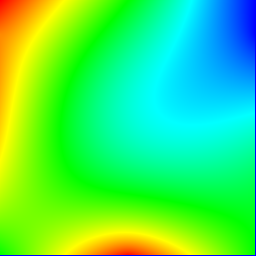
\includegraphics[width=\linewidth]{heat-jacobi-seq.png}
    \caption{Jacobi}
  \end{subfigure}
  \hspace{1cm}
  \begin{subfigure}{0.4\textwidth}
    \centering
    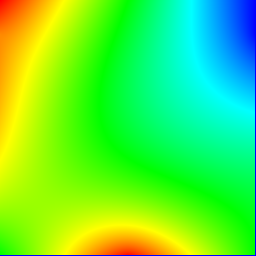
\includegraphics[width=\linewidth]{heat-gauss-seq.png}
    \caption{Gauss-Seidel}
  \end{subfigure}
  \caption{Images generated by the sequential code (\texttt{heat-seq}).}
  \label{fig:seq}
\end{figure}

% ================================================================
\section{Dependency analysis with Tareador}
% ================================================================

Tareador runs the program once sequentially. For every region we mark as a task, it records which memory addresses the task reads and writes. If one task writes an address that another reads or writes (or reads an address that another writes), Tareador adds a dependency edge between them. From the resulting task dependency graph (TDG) it simulates the parallel execution on $N$ processors, which gives an upper bound on the speedup of each task decomposition, without any runtime overheads.

The analysis uses the small problem from \texttt{run-tareador.sh} (\texttt{-s 32 -n 4}: a $32\times32$ body and 4 iterations). The accumulation into \texttt{sum} is excluded with \texttt{tareador\_disable\_object(\&sum)}. Otherwise every task would depend on the previous one through \texttt{sum +=}; in the OpenMP code this conflict is resolved with a \texttt{reduction}.

\subsection{Jacobi}

We explored three task decompositions:
\begin{description}
  \item[J1 (coarse):] one task per call to \texttt{solve} (\texttt{jacobi}) and one per call to \texttt{copy\_mat}. These are the default tasks in \texttt{heat-tareador.c}.
  \item[J2 (blocks in \texttt{solve}):] J1 plus the \texttt{solve(\%d,\%d)} tasks in \texttt{solver-tareador.c}. Each call to \texttt{solve} is split into $4\times4=16$ block tasks; \texttt{copy\_mat} remains a single task.
  \item[J3 (blocks in \texttt{solve} and \texttt{copy\_mat}):] J2 plus the \texttt{copy(\%d,\%d)} tasks, so the copy is also split into 16 block tasks.
\end{description}

\paragraph{Task dependency graphs.}
In J1 (Figure~\ref{fig:tdg-coarse}) the tasks form a single chain: \texttt{jacobi} $\rightarrow$ \texttt{copy\_mat} $\rightarrow$ \texttt{jacobi} $\rightarrow \dots$
\begin{itemize}
  \item \texttt{copy\_mat} reads \texttt{uhelp}, which \texttt{solve} has just written.
  \item The next \texttt{solve} reads \texttt{u}, which \texttt{copy\_mat} has just written.
\end{itemize}
The edges from each \texttt{jacobi} task back to the main program correspond to \texttt{residual}, which the \texttt{while} loop must read before starting the next iteration. The iterations of the main loop are therefore inherently sequential, and any parallelism has to come from inside each iteration.

In J2 and J3 (Figure~\ref{fig:tdg-blocks}) there are \emph{no edges between the 16 \texttt{solve} blocks}. Each block reads \texttt{u} and writes only its own part of \texttt{uhelp}, so the blocks are independent. The same holds for the 16 \texttt{copy} blocks in J3. Between the phases there is a single edge (\texttt{jacobi} $\rightarrow$ \texttt{copy\_mat} $\rightarrow$ \texttt{jacobi}), because the block tasks are nested inside the coarse tasks: every block of one phase must finish before any block of the next phase can start.

\begin{figure}[H]
  \centering
  
\includegraphics[height=0.55\textheight]{jacobi_dg_coarse.pdf}
  \caption{TDG of version J1 (coarse tasks), 4 iterations: a fully sequential chain.}
  \label{fig:tdg-coarse}
\end{figure}

\begin{figure}[H]
  \centering
  \begin{subfigure}[t]{0.49\textwidth}
    \centering
    \includegraphics[width=\linewidth]{jacobi_dg_blocks_v1.pdf}
    \caption{J2: 16 \texttt{solve} blocks per iteration, \texttt{copy\_mat} as a single task.}
  \end{subfigure}
  \hfill
  \begin{subfigure}[t]{0.49\textwidth}
    \centering
    \includegraphics[width=\linewidth]{jacobi_dg_blocks_v2.pdf}
    \caption{J3: 16 \texttt{solve} blocks and 16 \texttt{copy} blocks per iteration.}
  \end{subfigure}
  \caption{TDGs of the block decompositions. There are no dependencies between blocks of the same phase.}
  \label{fig:tdg-blocks}
\end{figure}

\paragraph{Simulated parallel execution.}
Table~\ref{tab:tareador-jacobi} shows the simulated execution time on 1, 4, 8 and 16 processors. Figures~\ref{fig:sim-coarse}--\ref{fig:sim-blocks2} show some of the timelines.

\begin{table}[H]
\centering
\begin{tabular}{lrrrr}
\toprule
Version & 1 proc. & 4 proc. & 8 proc. & 16 proc. \\
\midrule
J1 coarse          & 553.5 ms & 553.4 ms & 553.4 ms & 553.4 ms \\
                   & 1.00     & 1.00     & 1.00     & 1.00 \\
J2 blocks (solve)  & 553.7 ms & 264.1 ms & 216.5 ms & 196.1 ms \\
                   & 1.00     & 2.10     & 2.56     & 2.82 \\
J3 blocks (solve + copy) & 553.9 ms & 142.8 ms & 75.4 ms & 46.3 ms \\
                   & 1.00     & 3.88     & 7.34     & 11.96 \\
\bottomrule
\end{tabular}
\caption{Tareador simulation: simulated time (first row of each version) and speedup with respect to 1 processor (second row).}
\label{tab:tareador-jacobi}
\end{table}

\begin{itemize}
  \item \textbf{J1} has no parallelism at all. Figure~\ref{fig:sim-coarse} shows a staircase where only one processor is busy at any time, so the speedup is 1 for any number of processors.
  \item \textbf{J2} parallelises \texttt{solve}, but \texttt{copy\_mat} runs on a single processor while all the others are idle: the long cyan bar in Figure~\ref{fig:sim-blocks1}. The copy is $4 \times 41\,010 = 164\,040$ of the $553\,718$ instructions, a serial fraction of $f \approx 0.30$. Amdahl's law limits the speedup to $1/f \approx 3.4$, and to $1/(0.30 + 0.70/16) \approx 2.9$ on 16 processors, close to the simulated 2.82. Parallelising only the solver is therefore not enough.
  \item \textbf{J3} also parallelises the copy and scales almost linearly up to 8 processors (97\% efficiency on 4 and 92\% on 8), reaching $11.96\times$ on 16. It does not reach 16 for three reasons. First, the blocks have different sizes: border blocks skip the boundary rows and columns, so for example \texttt{solve\_3\_3} executes 4\,689 instructions against 7\,543 for \texttt{solve\_1\_1}. Second, there is a barrier between the \texttt{solve} and \texttt{copy} phases. Third, the parent tasks spend some time creating their 16 children (the bundles of yellow lines at the start of each phase).
\end{itemize}

In the timelines, the yellow lines are the task creation and synchronisation edges drawn by the simulator: from the parent to its children at the start of each phase, and from the children to the join at the end. The green flags mark the start and end events of each task.

\begin{figure}[H]
  \centering
  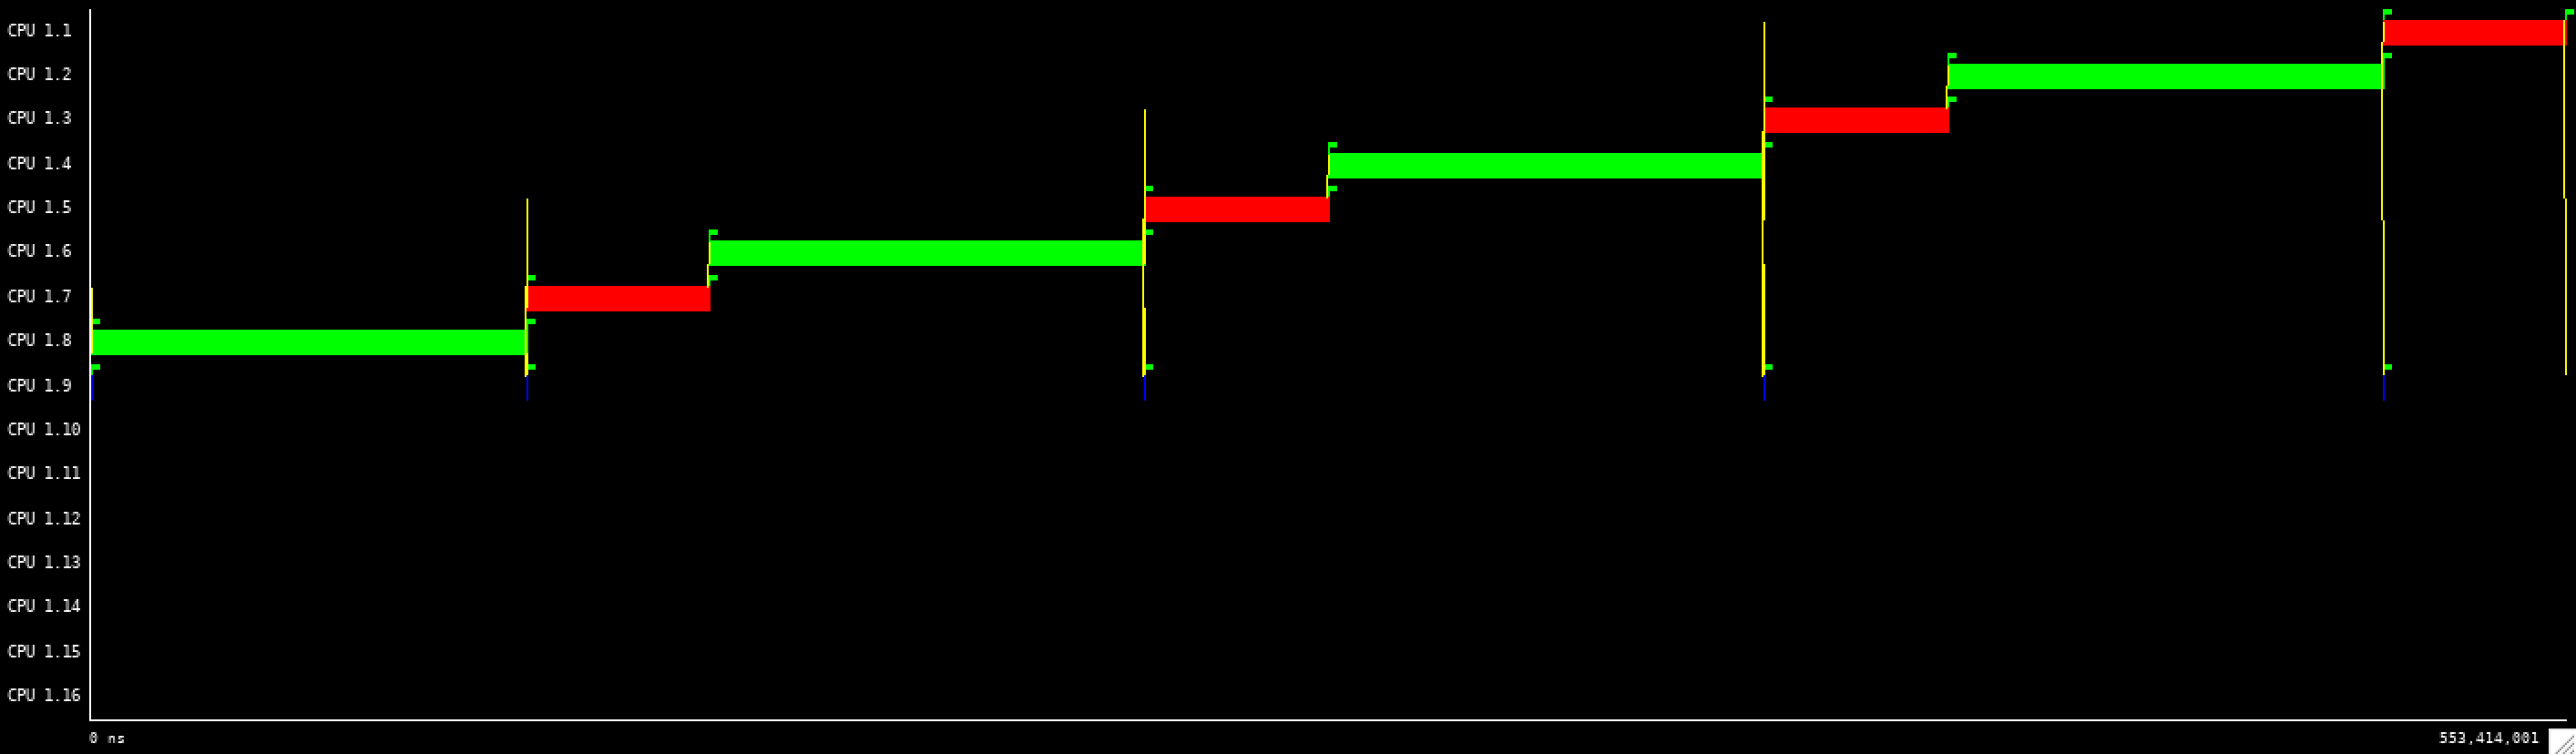
\includegraphics[width=0.9\textwidth]{jacobi_coarse_16cores.png}
  \caption{J1, 16 processors: \texttt{jacobi} (green) and \texttt{copy\_mat} (red) never overlap.}
  \label{fig:sim-coarse}
\end{figure}

\begin{figure}[H]
  \centering
  \begin{subfigure}{\textwidth}
    \centering
    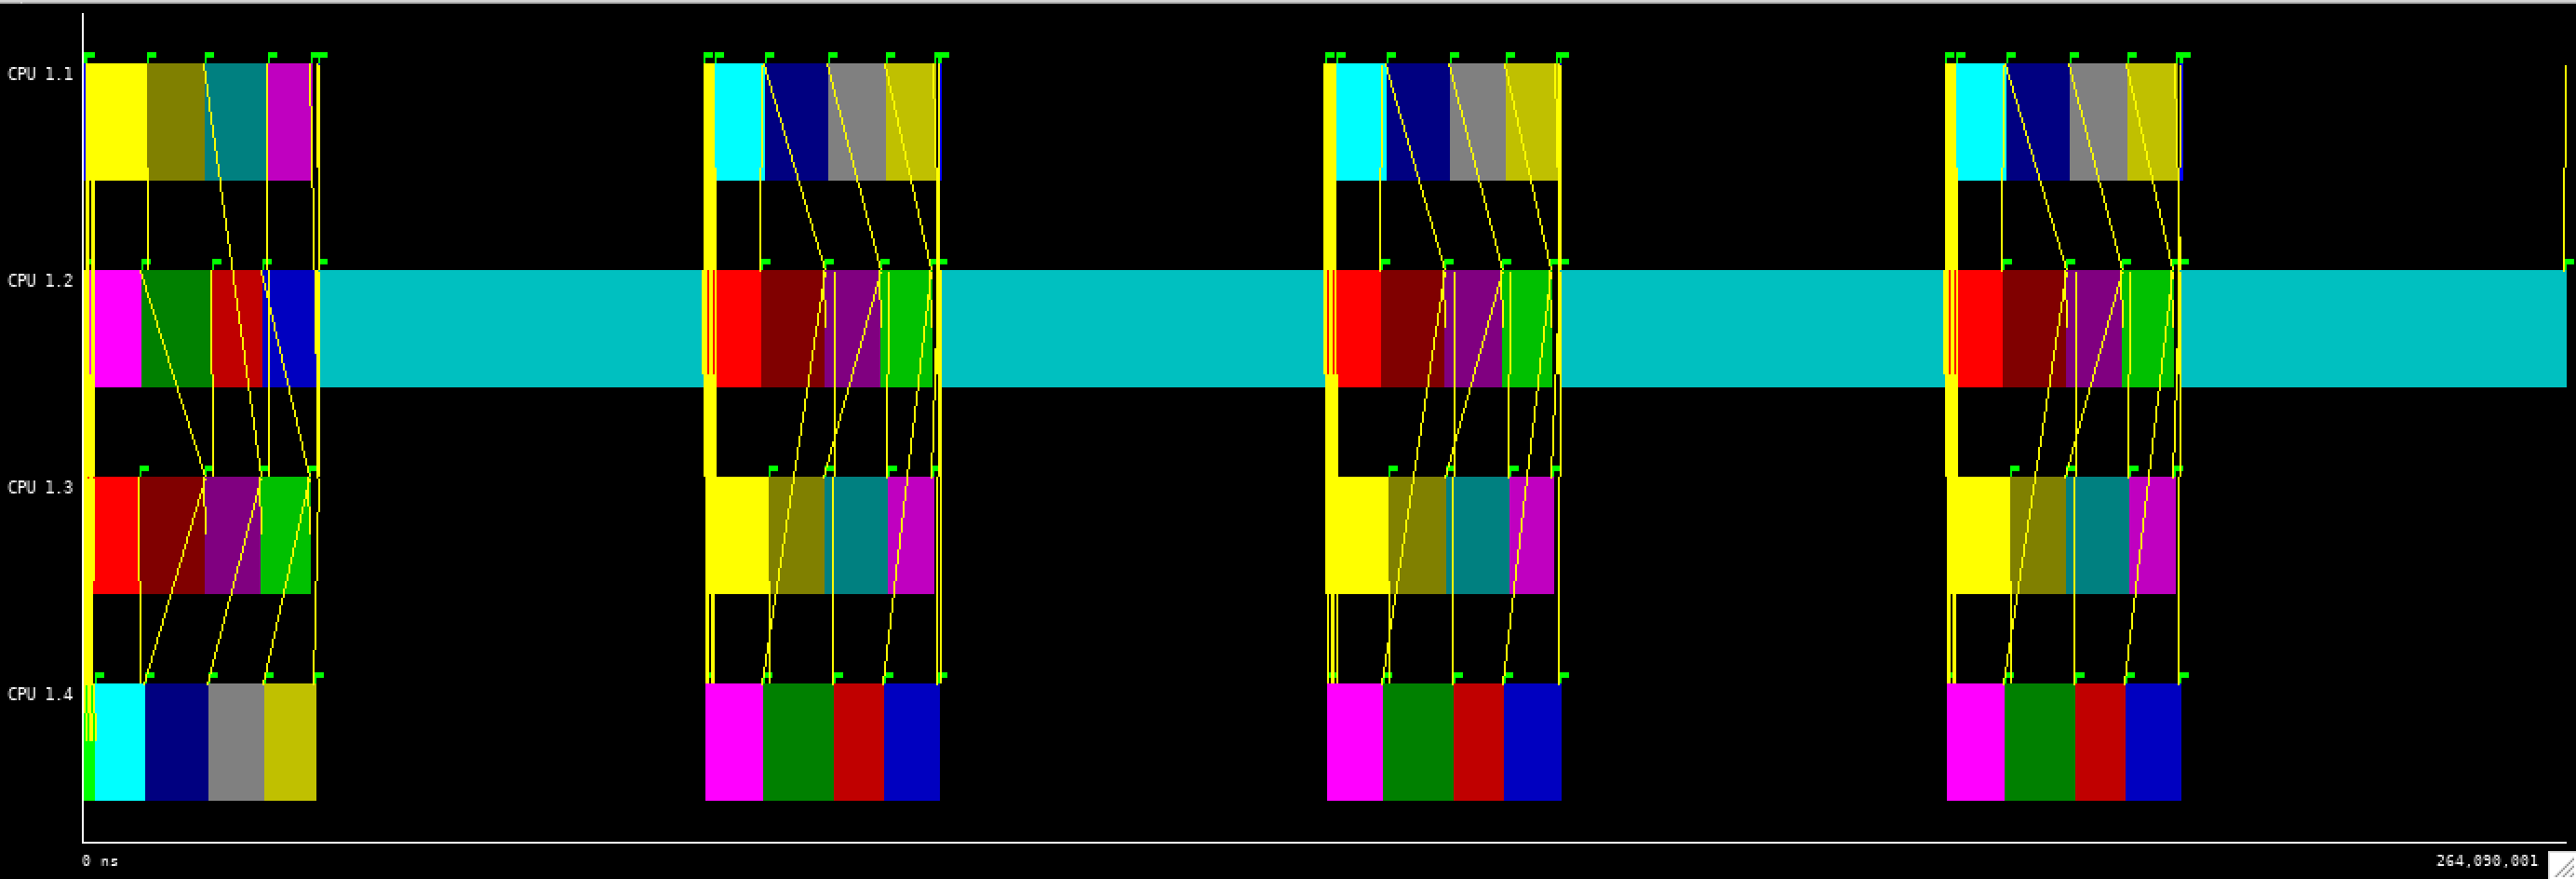
\includegraphics[width=0.9\textwidth]{jacobi_blocks01_4cores.png}
    \caption{4 processors}
  \end{subfigure}

  \vspace{2mm}
  \begin{subfigure}{\textwidth}
    \centering
    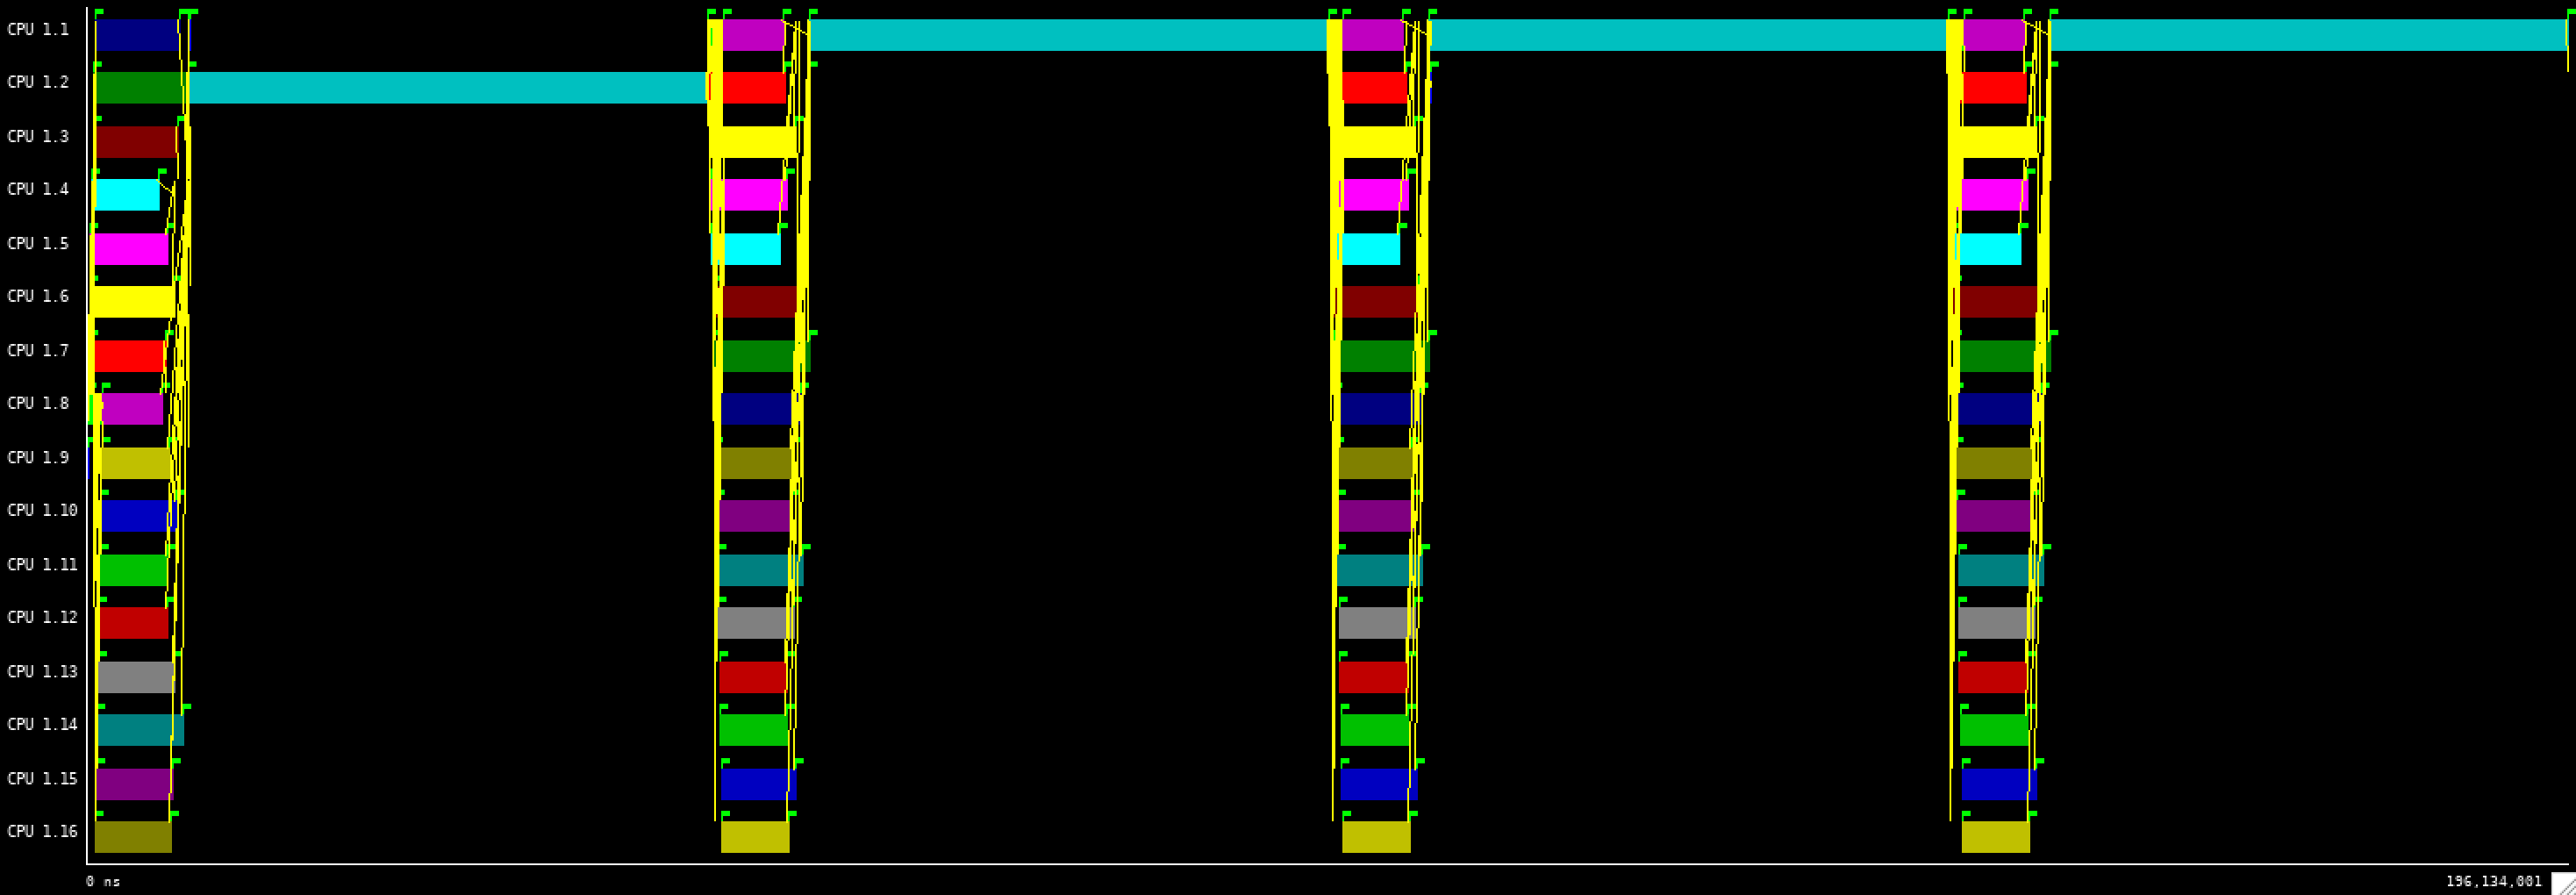
\includegraphics[width=0.9\textwidth]{jacobi_blocks01_16cores.png}
    \caption{16 processors}
  \end{subfigure}
  \caption{J2: the 16 \texttt{solve} blocks run in parallel, but \texttt{copy\_mat} (cyan) runs on a single processor while the others are idle.}
  \label{fig:sim-blocks1}
\end{figure}

\begin{figure}[H]
  \centering
  \begin{subfigure}{\textwidth}
    \centering
    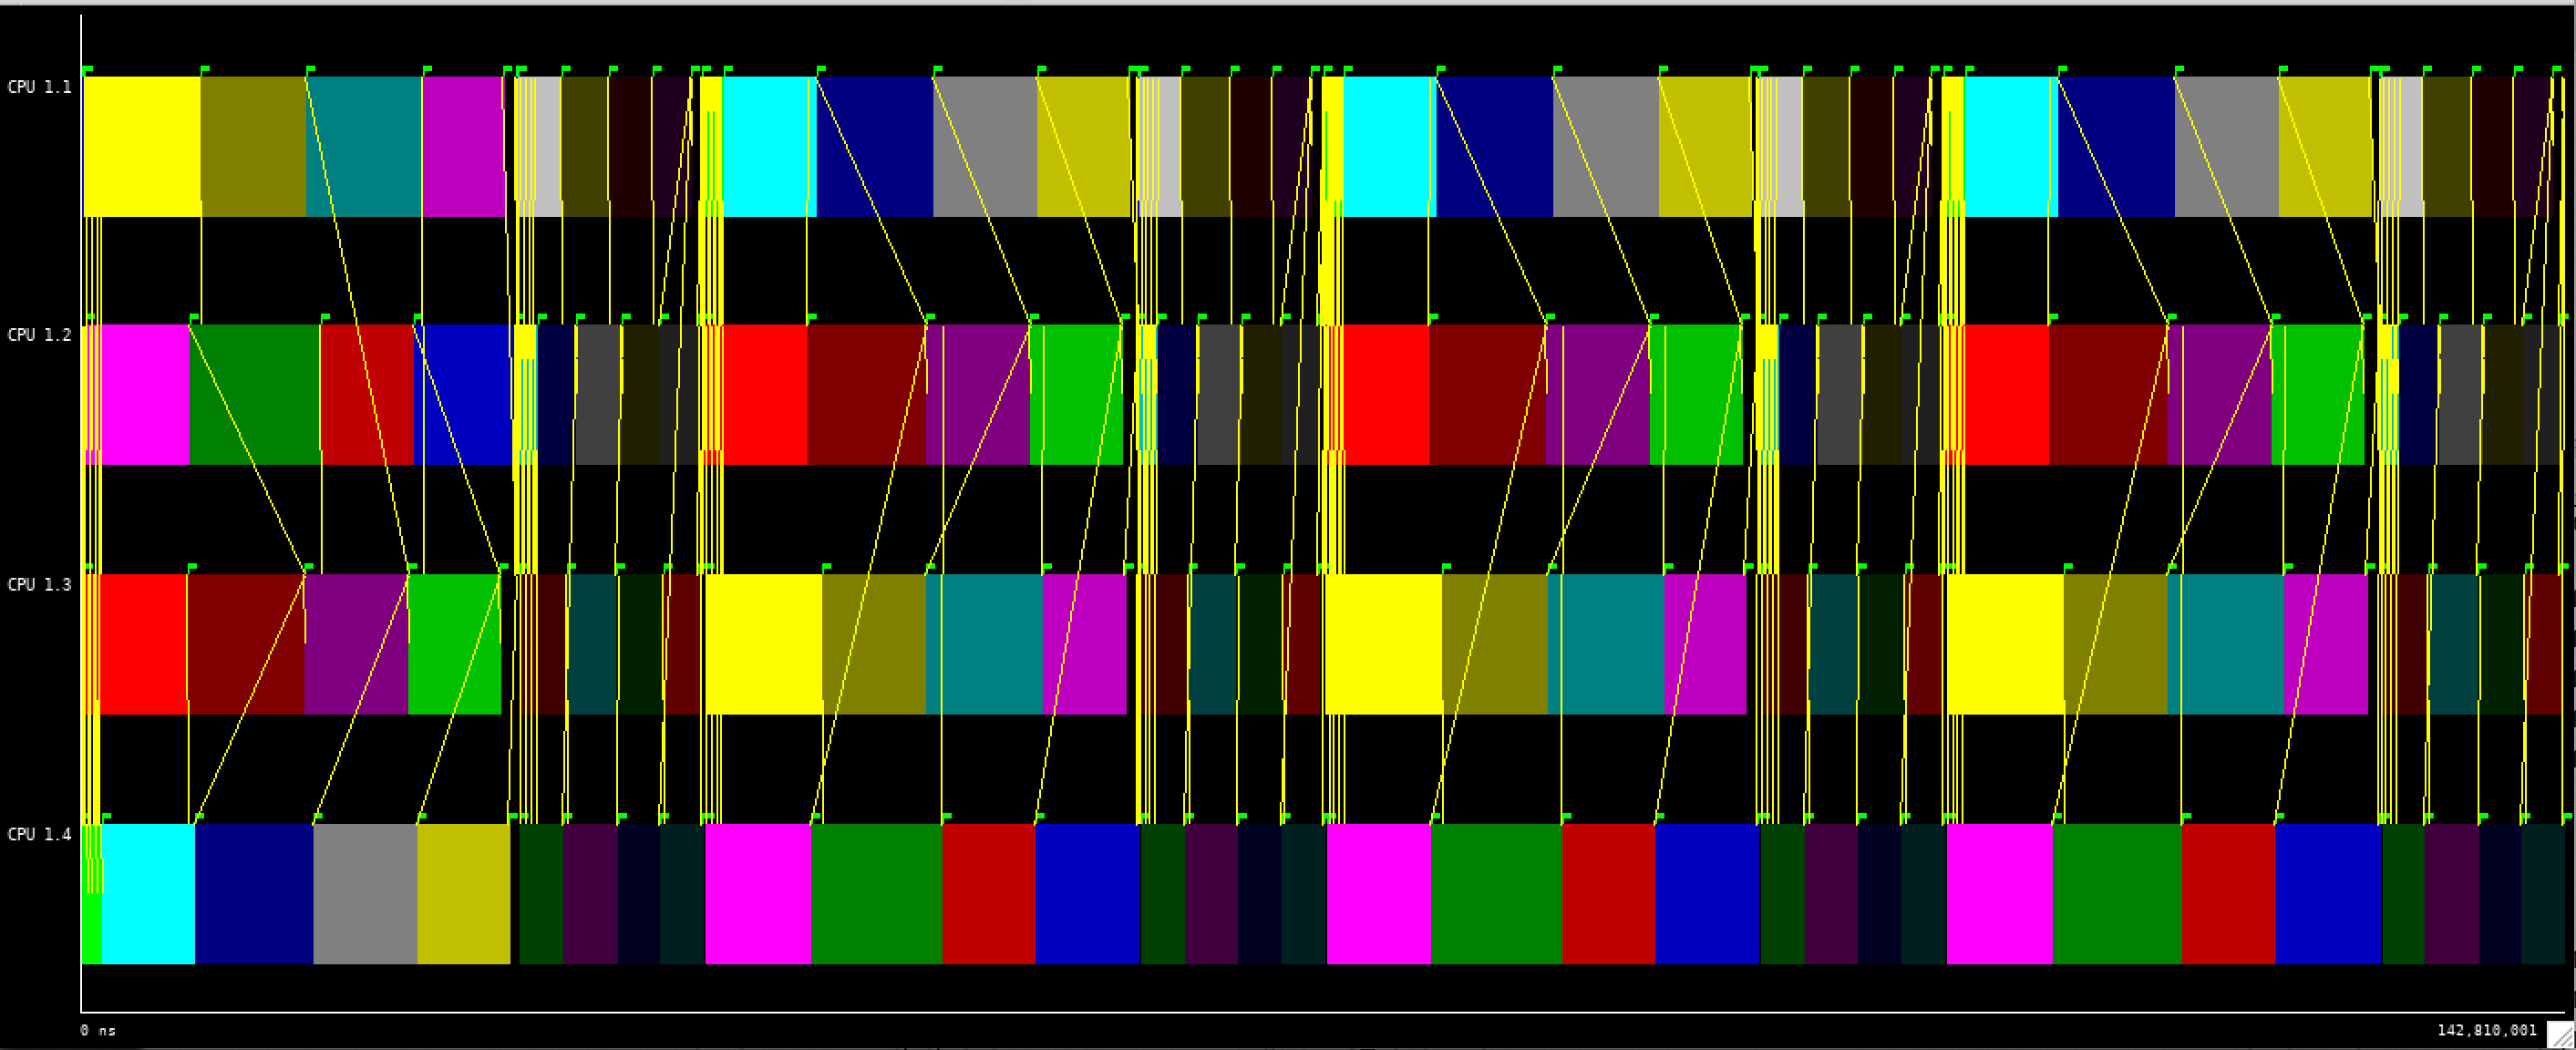
\includegraphics[width=0.9\textwidth]{jacobi_blocks02_4cores.png}
    \caption{4 processors}
  \end{subfigure}

  \vspace{2mm}
  \begin{subfigure}{\textwidth}
    \centering
    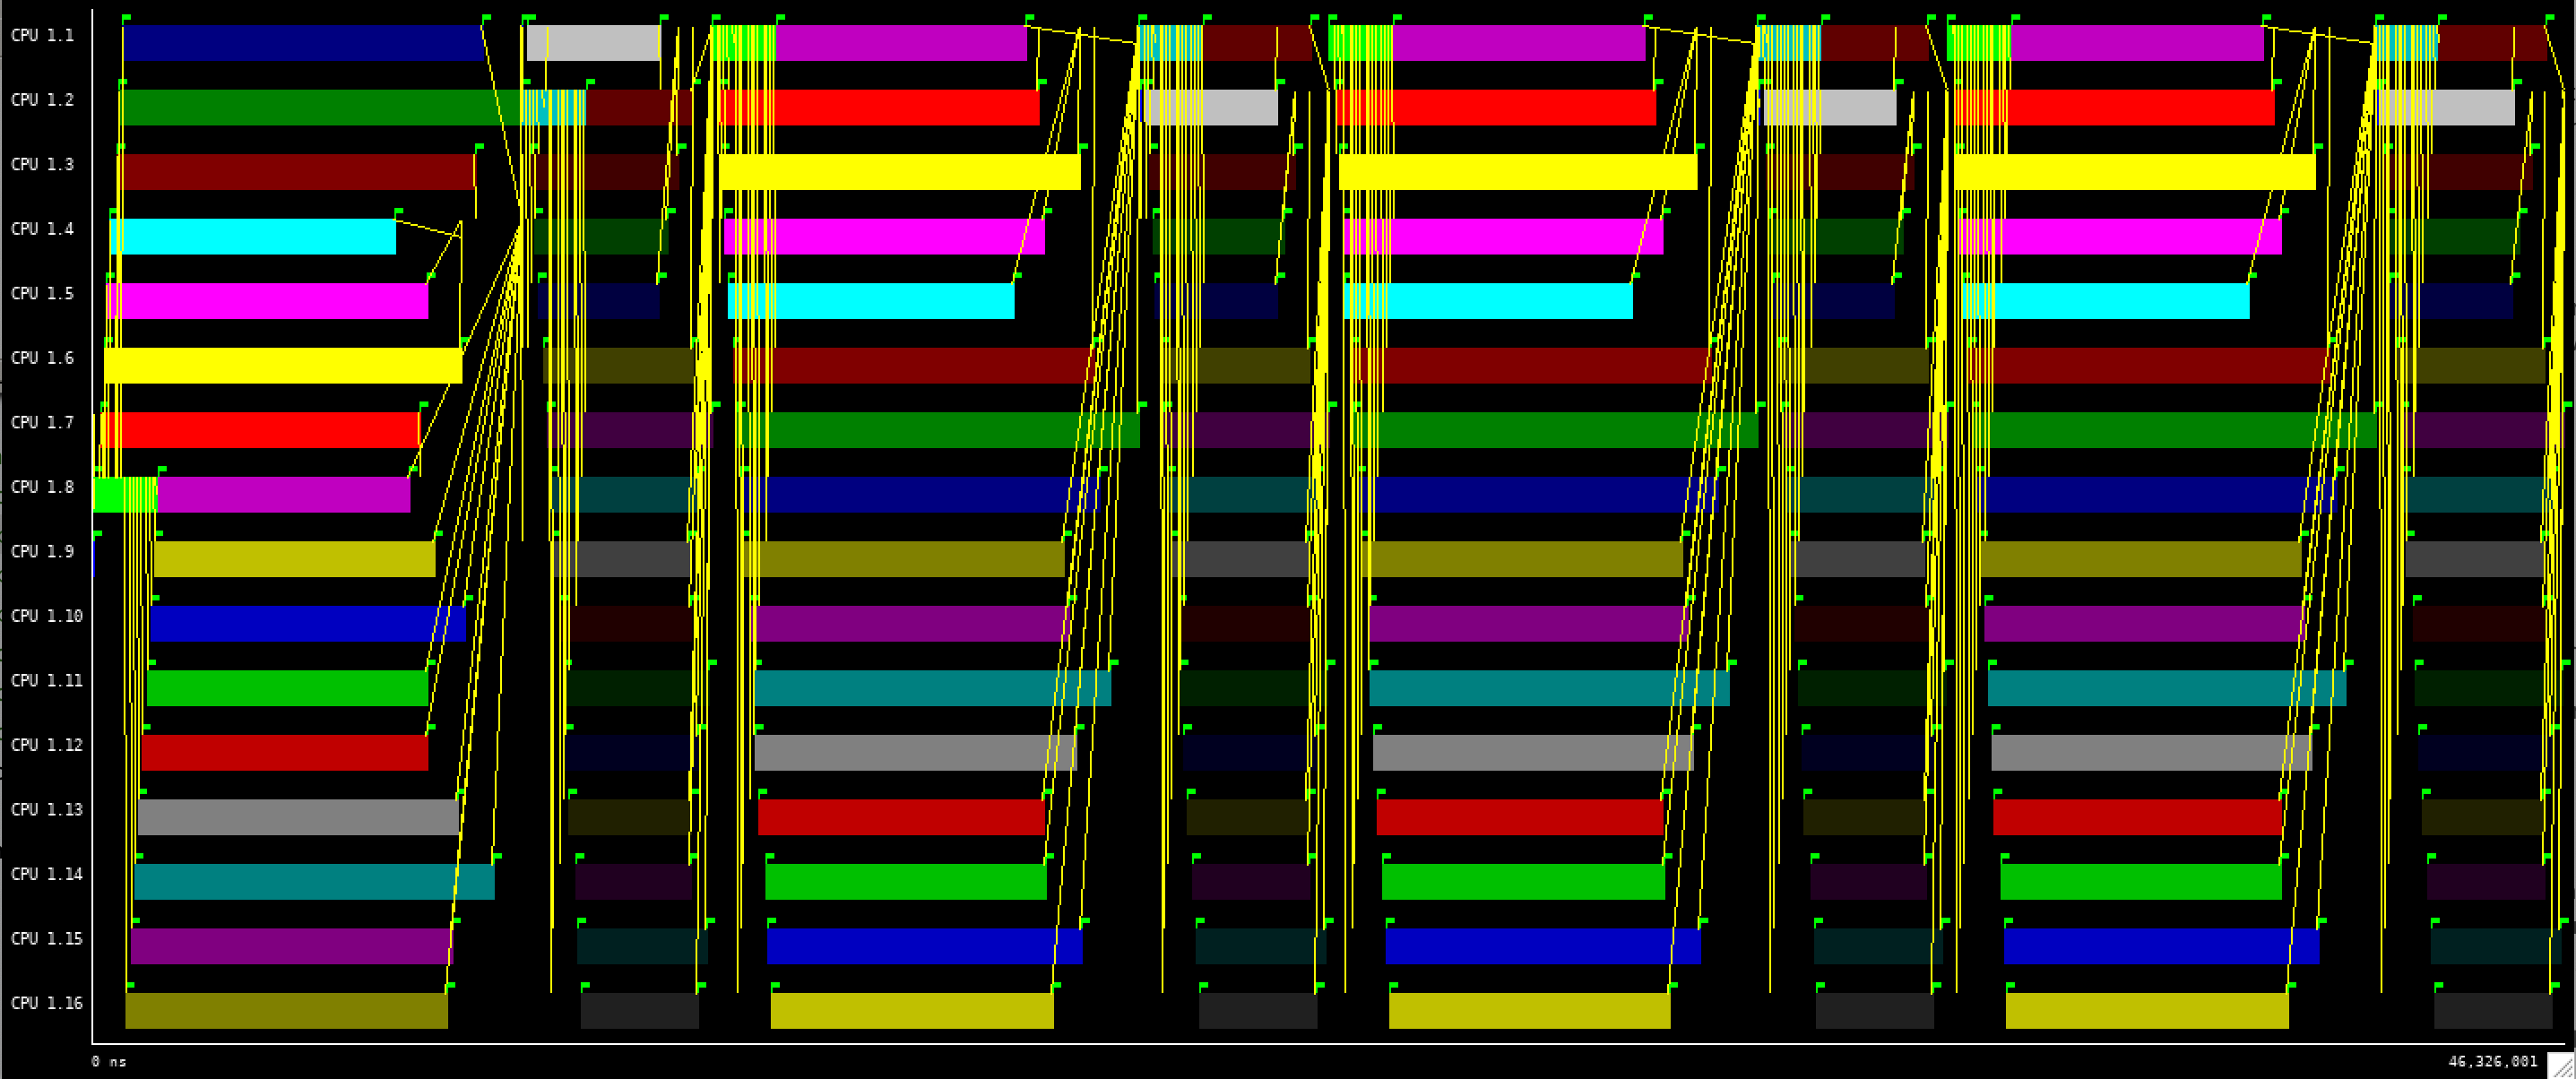
\includegraphics[width=0.9\textwidth]{jacobi_blocks02_16cores.png}
    \caption{16 processors}
  \end{subfigure}
  \caption{J3: both phases are parallel. The bright blocks are \texttt{solve} and the dark blocks are \texttt{copy}.}
  \label{fig:sim-blocks2}
\end{figure}

\paragraph{Conclusions for the OpenMP implementation.}
\begin{itemize}
  \item The parallelism is inside each iteration, so the parallel region must be inside \texttt{solve} (and \texttt{copy\_mat}), not around the \texttt{while} loop.
  \item The rows of \texttt{solve} are independent, so each thread can process its own rows without locks.
  \item \texttt{sum} needs a reduction, and the temporaries \texttt{tmp} and \texttt{diff} must be private.
  \item The phases must be separated by a barrier. The implicit barrier at the end of each parallel region provides it.
  \item \texttt{copy\_mat} must also be parallelised. Otherwise it becomes the bottleneck, as in J2.
\end{itemize}

\subsection{Gauss-Seidel}

Gauss-Seidel updates \texttt{u} in place. To compute point $(i,j)$ it needs the \emph{new} values of the point above, $(i-1,j)$, and the point to the left, $(i,j-1)$, which have already been updated in the current iteration. It also needs the \emph{old} values of the point below and the point to the right, which have not been updated yet. At block level, block $(b_i,b_j)$ must therefore wait for the block above, $(b_i-1,b_j)$, and the block to the left, $(b_i,b_j-1)$. This is what makes the blocking provided in the code necessary: without blocks there would be a single task and no parallelism.

We explored three task decompositions. The source code of each version is stored in the directory \texttt{src/tareador-gauss/}.
\begin{description}
  \item[G1 (coarse):] one task per call to \texttt{solve} (\texttt{gausseidel} in \texttt{heat-tareador.c}).
  \item[G2 (blocks):] G1 plus the 16 \texttt{solve(\%d,\%d)} block tasks, nested inside the \texttt{gausseidel} task. Each iteration must finish before the next one starts, as in the real code, where \texttt{solve} returns the residual that the \texttt{while} loop checks.
  \item[G3 (blocks, no barrier):] only the 16 block tasks, without the outer \texttt{gausseidel} task. Consecutive iterations are allowed to overlap.
\end{description}

\paragraph{Task dependency graphs.}
G1 (Figure~\ref{fig:tdg-gauss}a) is again a sequential chain: each iteration reads and writes all of \texttt{u}. In G2 (Figure~\ref{fig:tdg-gauss}b), unlike Jacobi, \emph{there are dependencies between the blocks of the same iteration}: every block has incoming edges from the block above and the block to the left. The blocks that can run at the same time are those on the same anti-diagonal ($b_i+b_j$ constant). With $4\times4$ blocks, the parallelism within one iteration grows $1\to2\to3\to4$ and then decreases $4\to3\to2\to1$ (a wavefront). In G3 (Figure~\ref{fig:tdg-gauss-nb}) the iterations are no longer separated. Block $(0,0)$ of iteration $t+1$ only waits for blocks $(0,1)$ and $(1,0)$ of iteration $t$, which must read its old values before it overwrites them. The wavefronts of consecutive iterations therefore overlap, producing the diamond-shaped graph.

\begin{figure}[H]
  \centering
  \begin{subfigure}[t]{0.3\textwidth}
    \centering
    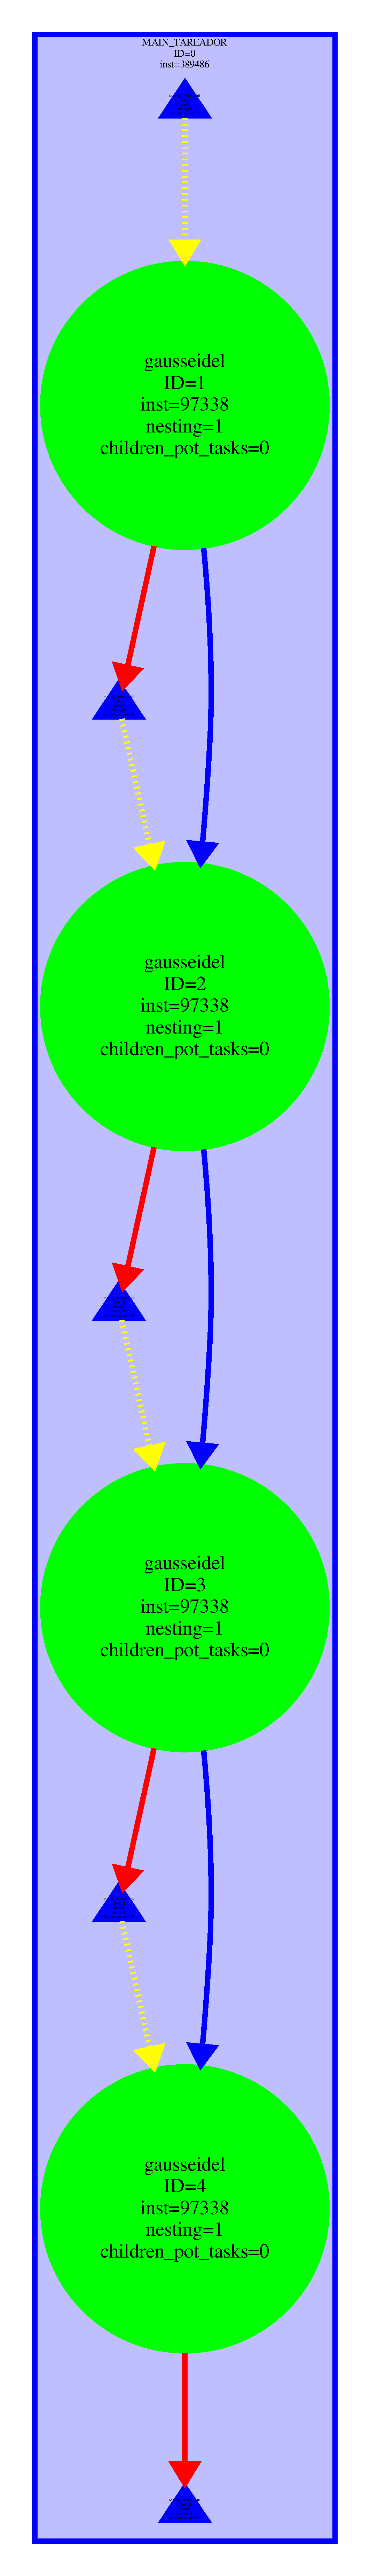
\includegraphics[height=0.5\textheight]{gauss_dg_coarse.pdf}
    \caption{G1 (coarse)}
  \end{subfigure}
  \hspace{1cm}
  \begin{subfigure}[t]{0.3\textwidth}
    \centering
    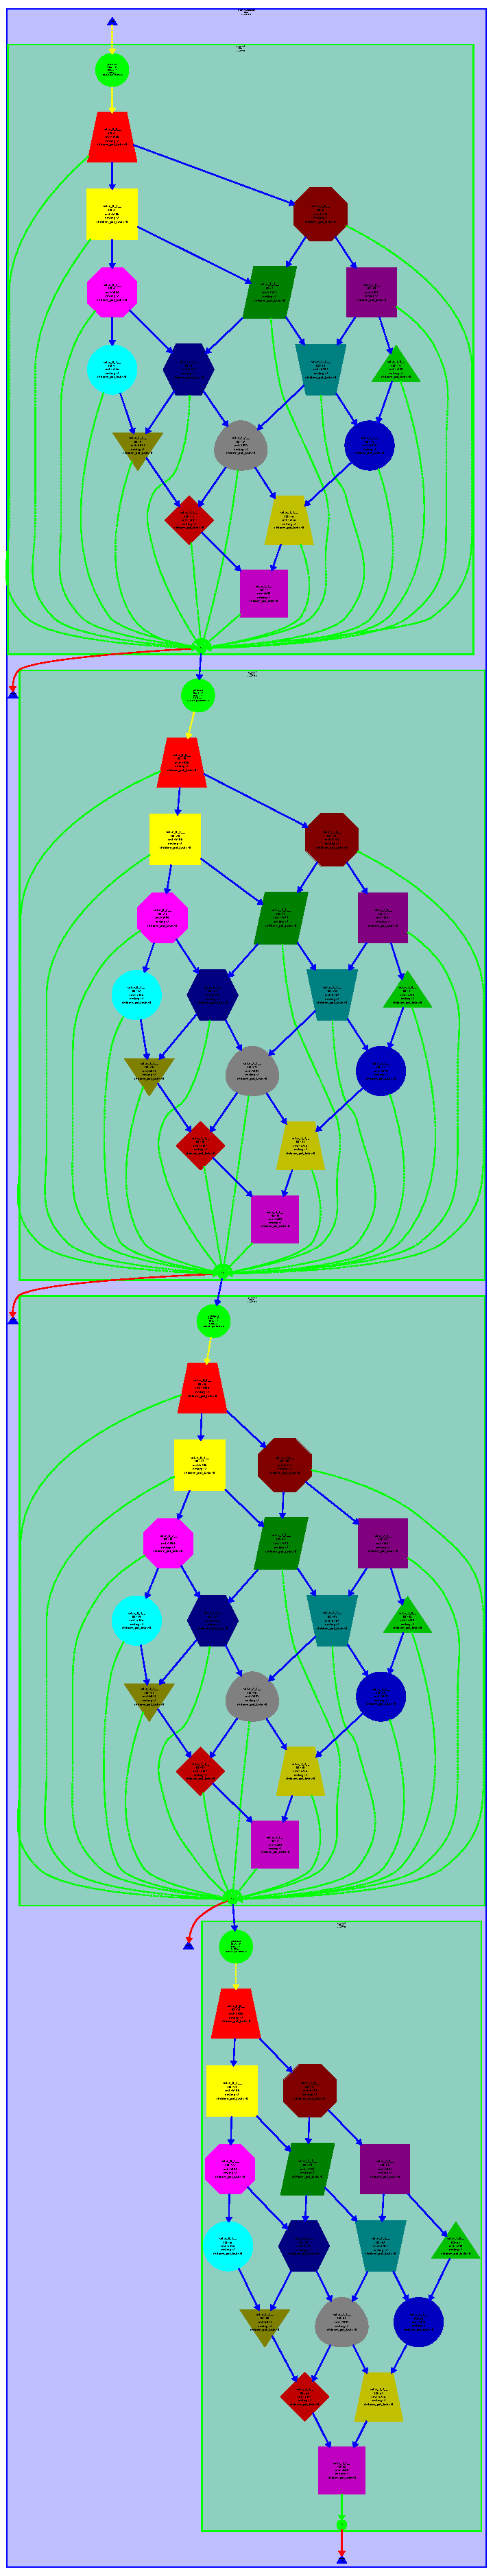
\includegraphics[height=0.5\textheight]{gauss_dg_blocks_small.pdf}
    \caption{G2 (blocks)}
  \end{subfigure}
  \caption{TDGs of Gauss-Seidel, 4 iterations. In G2 each iteration contains a wavefront of dependent blocks.}
  \label{fig:tdg-gauss}
\end{figure}

\begin{figure}[H]
  \centering
  \includegraphics[width=0.7\textwidth]{gauss_dg_blocks_nobarrier.pdf}
  \caption{TDG of G3 (blocks, no barrier between iterations): the wavefronts of consecutive iterations overlap.}
  \label{fig:tdg-gauss-nb}
\end{figure}

\paragraph{Simulated parallel execution.}
Table~\ref{tab:tareador-gauss} shows the simulated time on 1, 4, 8 and 16 processors. Figures~\ref{fig:sim-gauss-coarse}--\ref{fig:sim-gauss-nb} show some of the timelines.

\begin{table}[H]
\centering
\begin{tabular}{lrrrr}
\toprule
Version & 1 proc. & 4 proc. & 8 proc. & 16 proc. \\
\midrule
G1 coarse            & 389.5 ms & 389.5 ms & 389.5 ms & 389.5 ms \\
                     & 1.00     & 1.00     & 1.00     & 1.00 \\
G2 blocks            & 389.7 ms & 172.9 ms & 172.9 ms & 172.9 ms \\
                     & 1.00     & 2.25     & 2.25     & 2.25 \\
G3 blocks, no barrier & 389.7 ms & 113.7 ms & 86.1 ms  & 86.1 ms \\
                     & 1.00     & 3.43     & 4.53     & 4.53 \\
\bottomrule
\end{tabular}
\caption{Tareador simulation of Gauss-Seidel: simulated time and speedup with respect to 1 processor. The 1-processor times correspond to the total number of instructions of each graph.}
\label{tab:tareador-gauss}
\end{table}

\begin{itemize}
  \item \textbf{G1} has no parallelism (Figure~\ref{fig:sim-gauss-coarse}): one task at a time and a speedup of 1.
  \item \textbf{G2} reaches $2.25\times$ and does not improve beyond 4 processors. The critical path of one iteration crosses 7 blocks, for example $(0,0)\to(0,1)\to(1,1)\to(1,2)\to(2,2)\to(2,3)\to(3,3)$, about 43\,k of the 97\,k instructions of the iteration. This bounds the speedup to about $97/43 \approx 2.3$. At most 4 blocks (one anti-diagonal) are ever ready at the same time, so processors 5 to 16 stay idle, and the 4, 8 and 16-processor executions take exactly the same time. Figure~\ref{fig:sim-gauss-blocks} shows the filling and draining of the wavefront in every iteration.
  \item \textbf{G3} reaches $4.53\times$. Each new wavefront starts about two block steps after the previous one, so the critical path of 4 iterations shrinks from $4\times7=28$ to about $7+3\times2=13$ block steps. It uses up to about 8 processors, so 16 processors give no further improvement. This overlap is \emph{not} possible in the real code, because the \texttt{while} loop must check the residual of an iteration before starting the next. G2 is therefore the realistic model, and G3 shows the cost of that barrier.
\end{itemize}

The main conclusion is that the parallelism of Gauss-Seidel is limited by the number of blocks on an anti-diagonal and by the fill and drain of the wavefront in each iteration. Increasing the number of blocks in the $j$ dimension (Section~5.3) shortens these phases relative to the total, and is the only way to use more threads.

\begin{figure}[H]
  \centering
  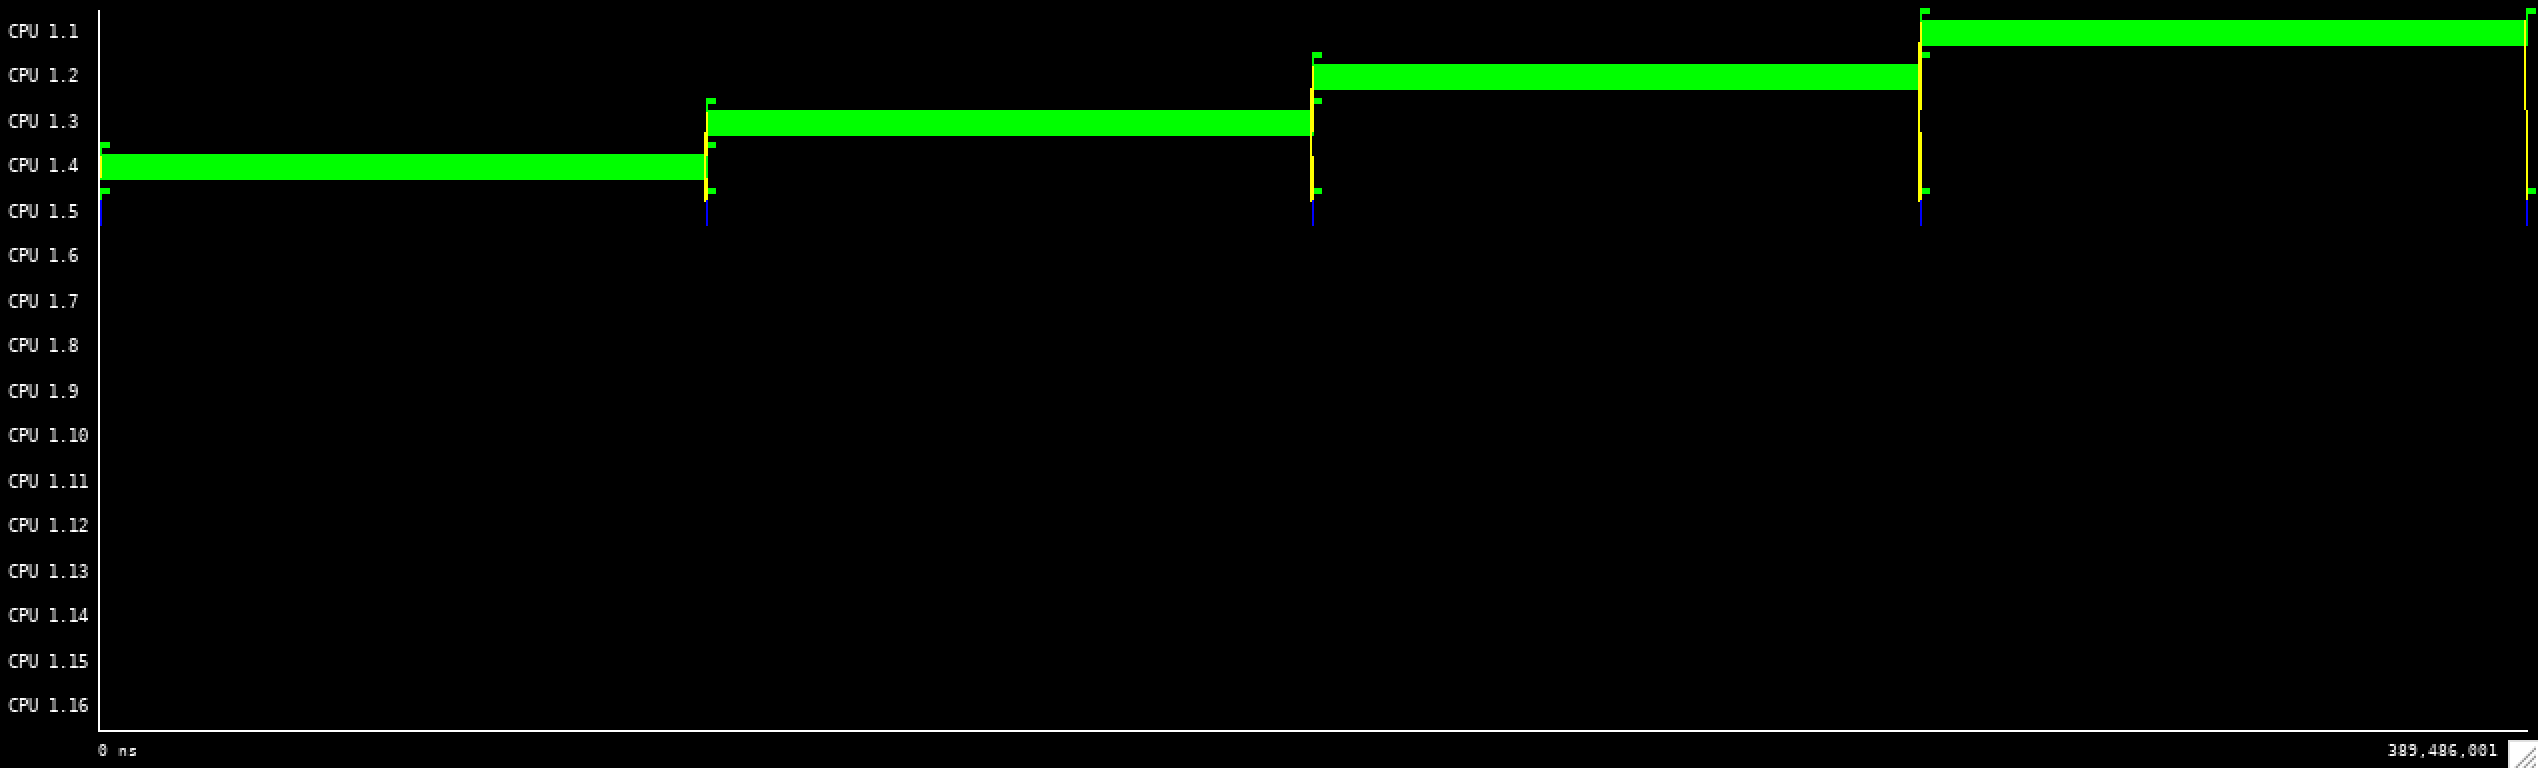
\includegraphics[width=0.9\textwidth]{gauss_coarse_16cores.png}
  \caption{G1, 16 processors: one \texttt{gausseidel} task at a time.}
  \label{fig:sim-gauss-coarse}
\end{figure}

\begin{figure}[H]
  \centering
  \begin{subfigure}{\textwidth}
    \centering
    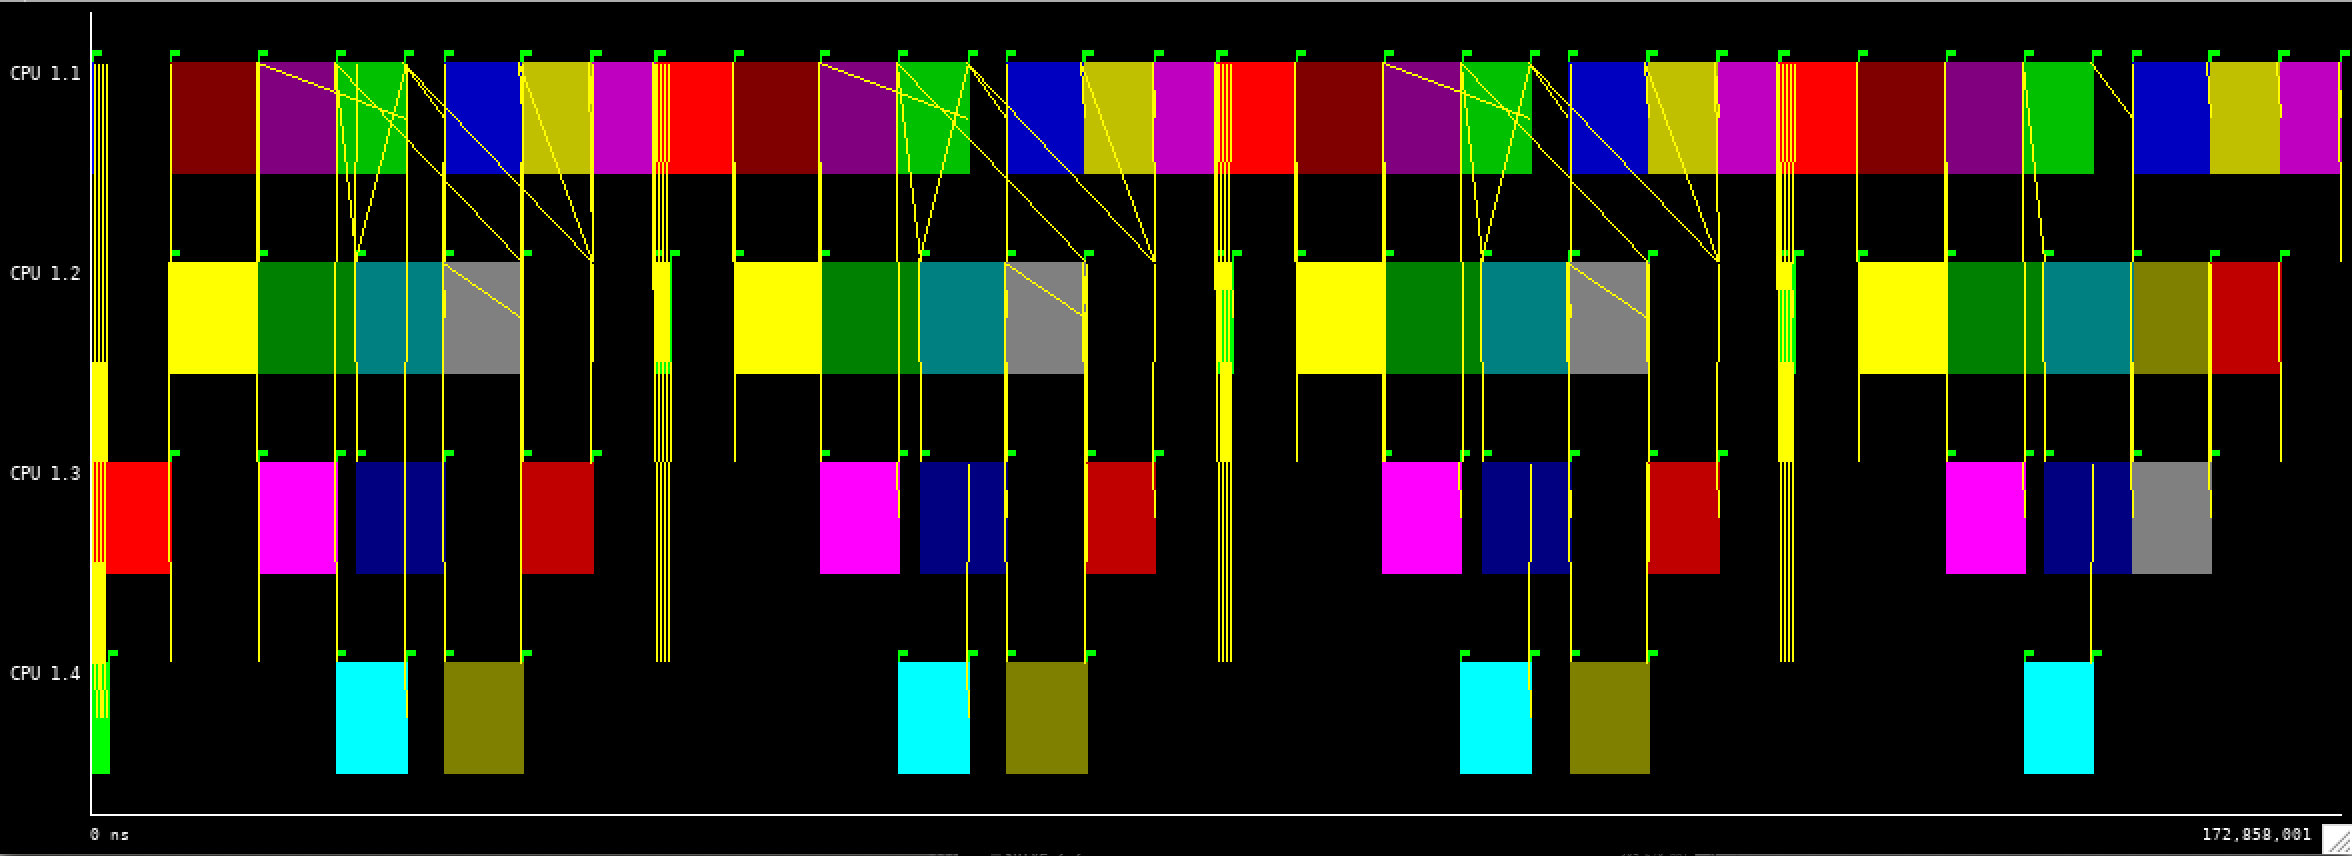
\includegraphics[width=0.9\textwidth]{gauss_blocks_4cores.png}
    \caption{4 processors}
  \end{subfigure}

  \vspace{2mm}
  \begin{subfigure}{\textwidth}
    \centering
    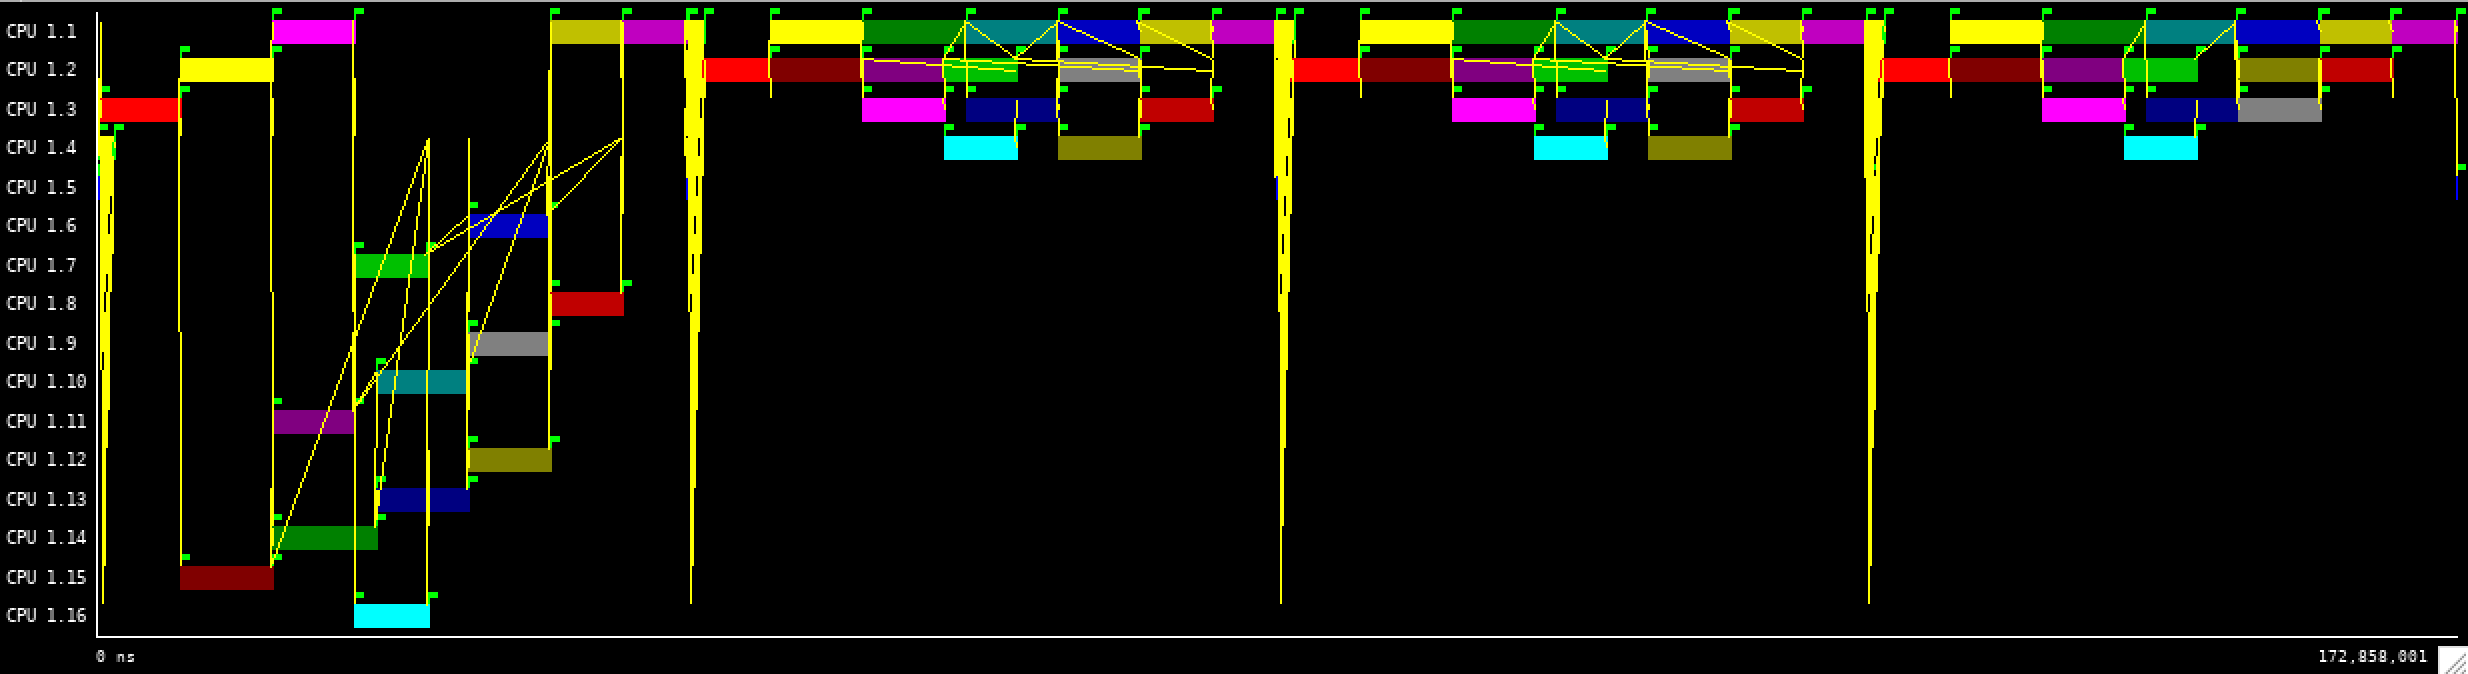
\includegraphics[width=0.9\textwidth]{gauss_blocks_16cores.png}
    \caption{16 processors: same time as with 4, at most 4 processors busy after the first iteration}
  \end{subfigure}
  \caption{G2: wavefront execution; parallelism fills and drains in every iteration.}
  \label{fig:sim-gauss-blocks}
\end{figure}

\begin{figure}[H]
  \centering
  \begin{subfigure}{\textwidth}
    \centering
    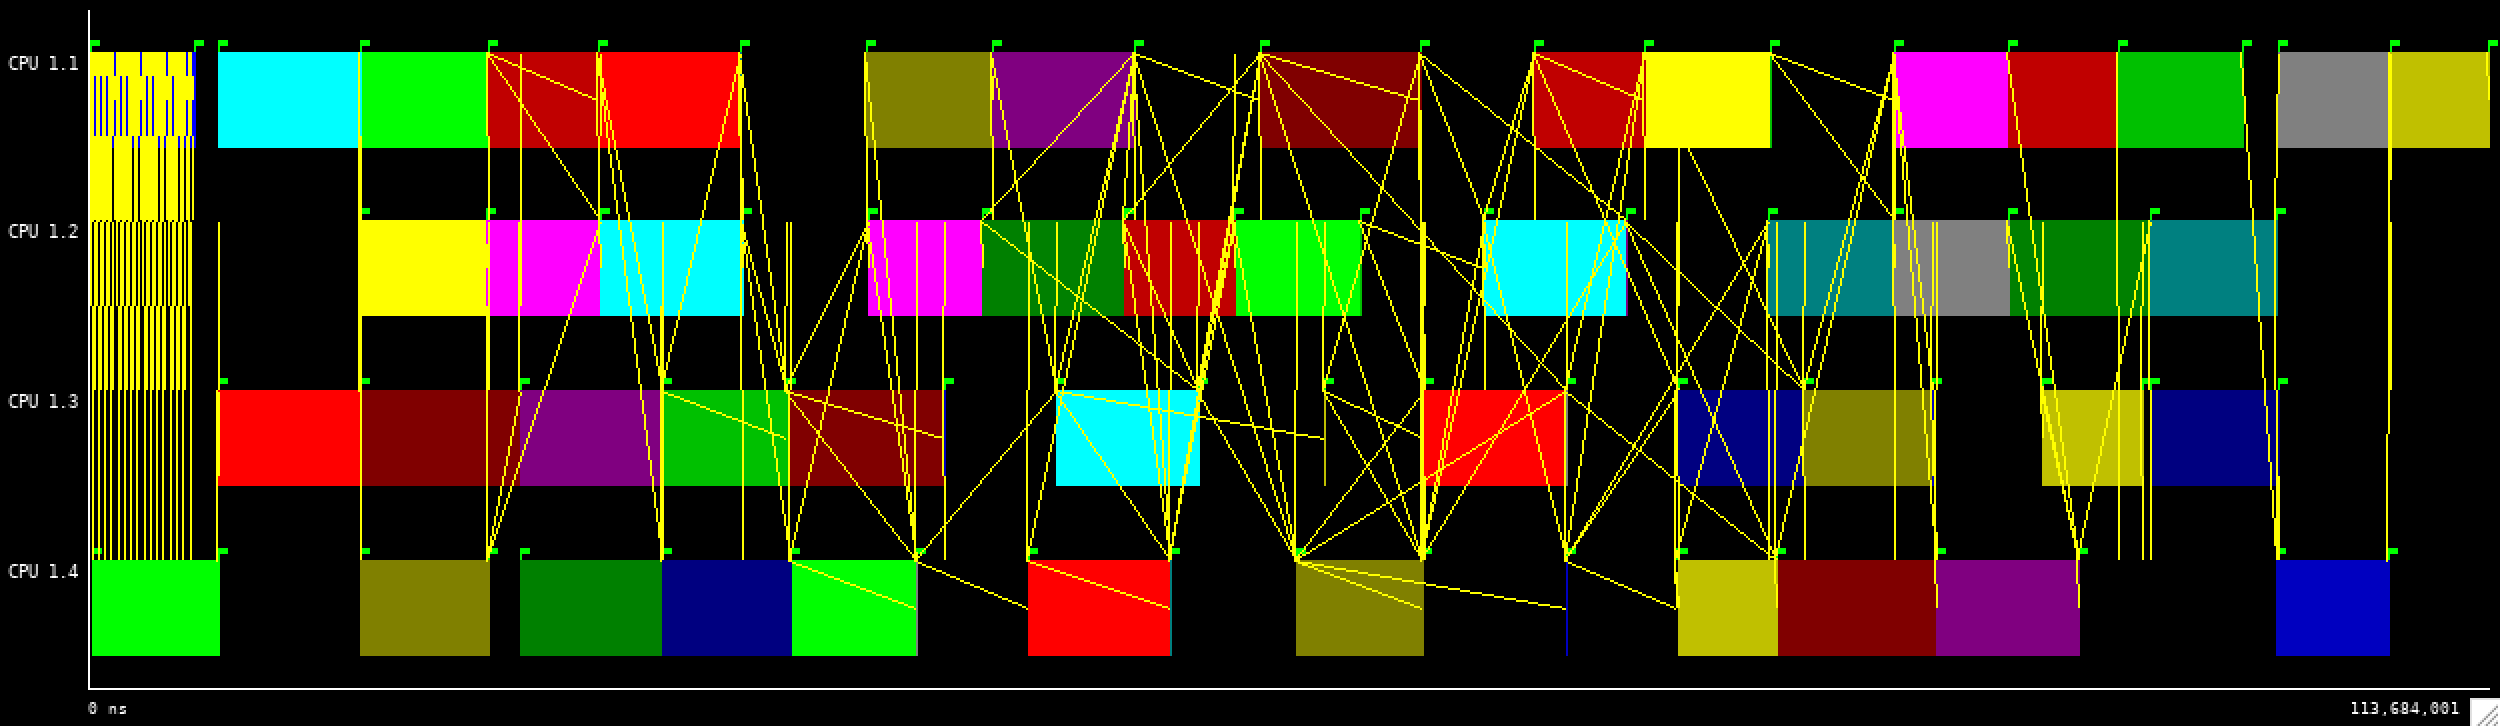
\includegraphics[width=0.9\textwidth]{gauss_blocks_nobarrier_4cores.png}
    \caption{4 processors}
  \end{subfigure}

  \vspace{2mm}
  \begin{subfigure}{\textwidth}
    \centering
    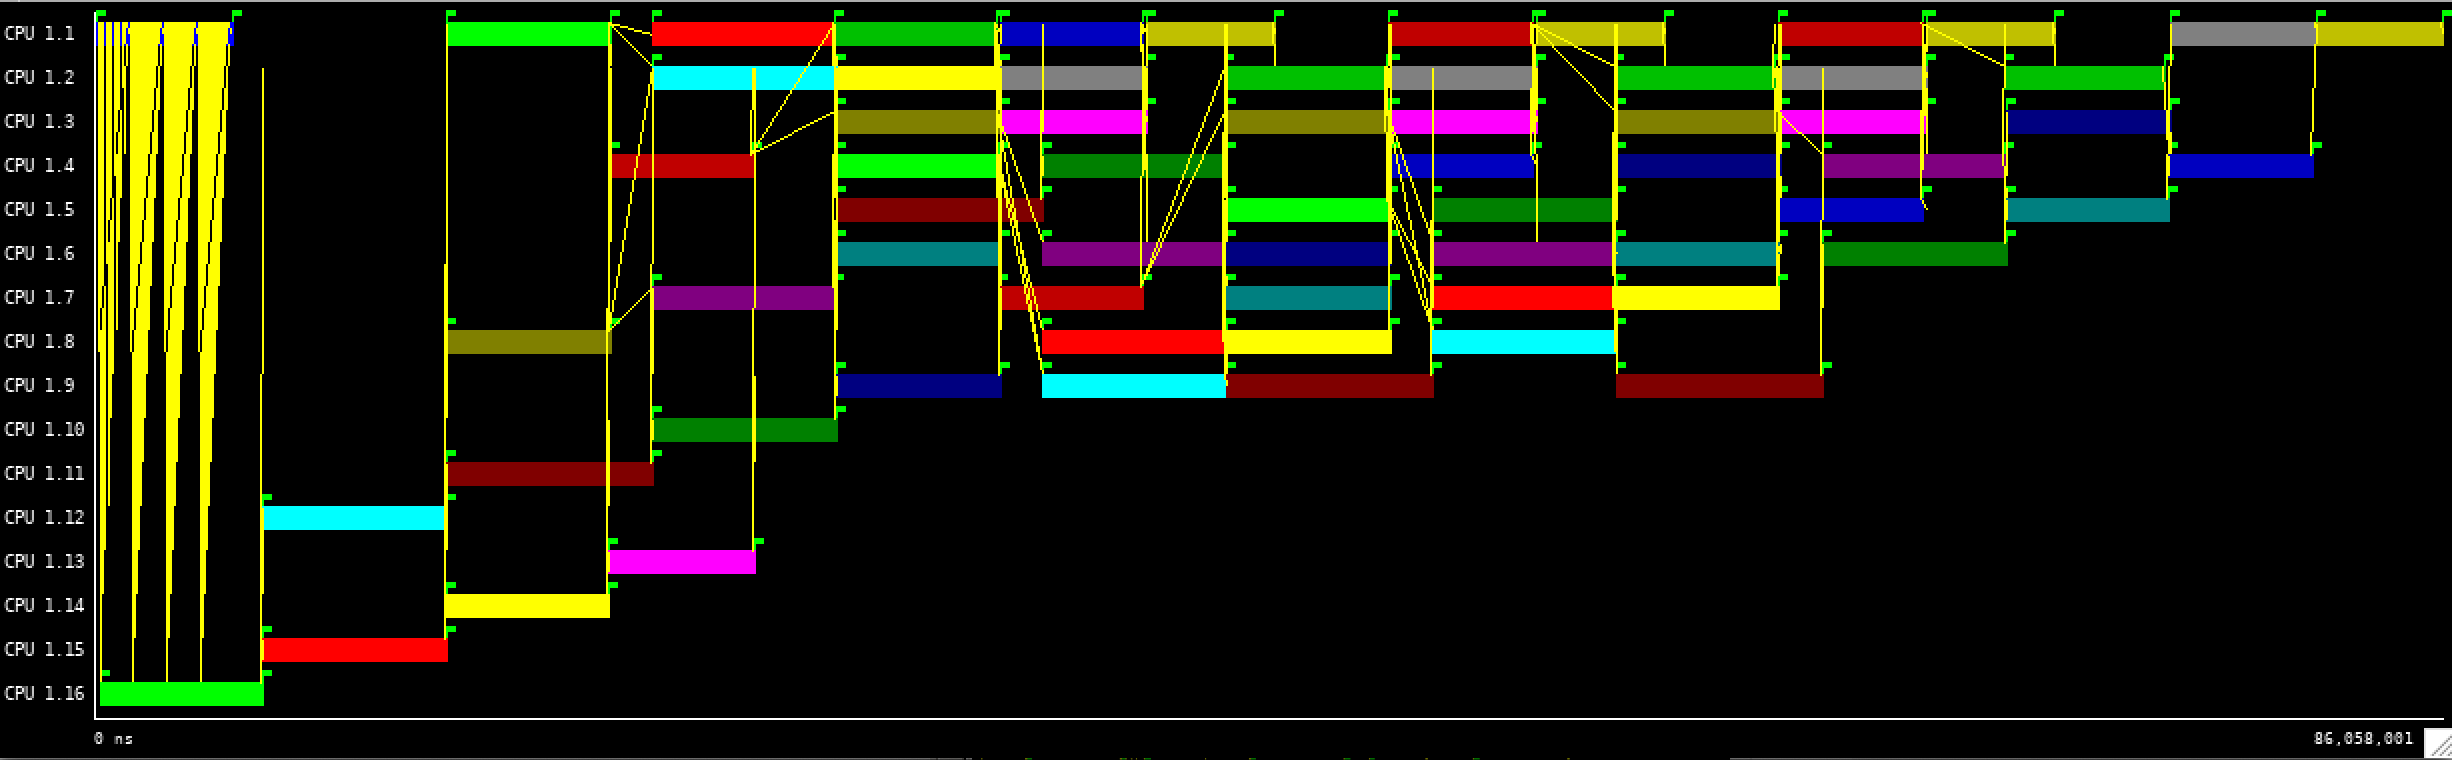
\includegraphics[width=0.9\textwidth]{gauss_blocks_nobarrier_16cores.png}
    \caption{16 processors}
  \end{subfigure}
  \caption{G3: without the barrier, consecutive iterations overlap and more processors are used.}
  \label{fig:sim-gauss-nb}
\end{figure}

% ================================================================
\section{Parallel Jacobi}
% ================================================================

\subsection{Data decomposition implementation}

The initial code in \texttt{solver-omp.c} is not correct:
\begin{lstlisting}
#pragma omp parallel     // complete data sharing constructs here
for (int i = 1; i < sizex - 1; i++)
    for (int j = 1; j < sizey - 1; j++) { ... sum += diff * diff; unew[...] = tmp; }
\end{lstlisting}
\texttt{\#pragma omp parallel} on its own does not distribute any work: every thread executes the complete loop. In addition, \texttt{tmp}, \texttt{diff} and \texttt{sum} are shared, so all threads overwrite the same temporaries (a data race), and the updates to \texttt{sum} are lost and counted multiple times. The residual is therefore wrong.

We completed the code following a geometric block decomposition by rows (Figure 4.1 of the assignment). Explicit work-sharing pragmas are not allowed, so each implicit task computes its own range of rows from \texttt{omp\_get\_thread\_num()} and \texttt{omp\_get\_num\_threads()}. We use the \texttt{lowerb}/\texttt{upperb} macros provided in the file, which also distribute the remainder rows when \texttt{sizex} is not a multiple of the number of threads. Clamping the range with \texttt{max(1, \dots)} and \texttt{min(sizex-2, \dots)} excludes the fixed boundary rows.

\begin{lstlisting}
double solve (double *u, double *unew, unsigned sizex, unsigned sizey) {
    double tmp, diff, sum = 0.0;

    if (u == unew) return solve_gauss(u, sizex, sizey);

    #pragma omp parallel private(tmp, diff) reduction(+:sum)
    {
        int myid  = omp_get_thread_num();
        int nthr  = omp_get_num_threads();
        int i_start = lowerb(myid, nthr, sizex);
        int i_end   = upperb(myid, nthr, sizex);

        for (int i = max(1, i_start); i <= min(sizex - 2, i_end); i++) {
            for (int j = 1; j < sizey - 1; j++) {
                tmp = 0.25 * ( u[ i * sizey       + (j - 1) ] +
                               u[ i * sizey       + (j + 1) ] +
                               u[ (i - 1) * sizey + j       ] +
                               u[ (i + 1) * sizey + j       ] );
                diff = tmp - u[i * sizey + j];
                sum += diff * diff;
                unew[i * sizey + j] = tmp;
            }
        }
    }
    return sum;
}
\end{lstlisting}

The clauses follow from the dependency analysis:
\begin{itemize}
  \item \texttt{private(tmp, diff)}: these are temporaries that are written before being read in every iteration, so each thread needs its own copy. Declaring them inside the loop would be equivalent.
  \item \texttt{reduction(+:sum)}: each thread accumulates into a private partial sum, and OpenMP combines the partial sums at the end of the region. This replaces the conflict on \texttt{sum} that we disabled in Tareador.
  \item No other synchronisation is needed. Each thread writes only its own rows of \texttt{unew} and only reads \texttt{u}. The implicit barrier at the end of the region guarantees that \texttt{copy\_mat} starts once all rows have been computed, and that the reduction has finished before \texttt{sum} is returned.
\end{itemize}

We call this version \textbf{v1}; \texttt{copy\_mat} is still sequential. We validated it with \texttt{submit-omp.sh} using 1 and 8 threads. The image is identical to the sequential one, and the number of iterations to convergence is the same.

\subsubsection{Overall analysis}

Table~\ref{tab:mf-v1} shows the \texttt{modelfactors} results of v1 (\texttt{-s 1022 -n 1000}).

\begin{table}[H]
\centering
\small
\begin{tabular}{|l|c|c|c|c|}
\hline
\multicolumn{5}{|c|}{Overview of whole program execution metrics} \\
\hline
\hline
Number of processors & 1 & 4 & 8 & 16 \\
\hline
Elapsed time (sec)      &       2.40 &       1.57 &       1.45 &       1.54 \\
\hline
Speedup                 &       1.00 &       1.52 &       1.65 &       1.56 \\
\hline
Efficiency              &       1.00 &       0.38 &       0.21 &       0.10 \\
\hline
\end{tabular}
\vspace{2mm}
\begin{tabular}{|l|c|c|c|c|}
\hline
\multicolumn{5}{|c|}{Overview of the Efficiency metrics in parallel fraction, $\phi$=73.59\%} \\
\hline
\hline
Number of processors & 1 & 4 & 8 & 16 \\
\hline
\hline
Global efficiency                      &     99.83\% &     83.82\% &     62.34\% &     35.50\% \\
\hline
\hline
Parallelization strategy efficiency &     99.83\% &     90.54\% &     98.52\% &     97.90\% \\
\hline
Load balancing                   &    100.00\% &     91.93\% &     99.87\% &     99.88\% \\
In execution efficiency          &     99.83\% &     98.50\% &     98.64\% &     98.02\% \\
\hline
\hline
Scalability for computation tasks   &    100.00\% &     92.57\% &     63.28\% &     36.27\% \\
\hline
IPC scalability                  &    100.00\% &     92.96\% &     67.93\% &     42.75\% \\
Instruction scalability          &    100.00\% &     99.98\% &     94.12\% &     85.89\% \\
Frequency scalability            &    100.00\% &     99.60\% &     98.97\% &     98.76\% \\
\hline
\end{tabular}
\vspace{2mm}
\begin{tabular}{|l|c|c|c|c|}
\hline
\multicolumn{5}{|c|}{Statistics about implicit or explicit tasks in parallel fraction} \\
\hline
\hline
Number of processors & 1 & 4 & 8 & 16 \\
\hline
\hline
Number of implicit tasks per thread (average us)    &          1000.0 &          1000.0 &          1000.0 &          1000.0 \\
\hline
Useful duration for implicit tasks (average us)     &         1762.37 &          475.96 &          348.13 &          303.73 \\
\hline
Load balancing for implicit tasks                &             1.0 &            0.92 &             1.0 &             1.0 \\
\hline
Time in synchronization implicit tasks (average us) &             0.0 &             0.0 &             0.0 &             0.0 \\
\hline
Time in fork/join implicit tasks (average us)       &            2.92 &           89.59 &             5.3 &            6.65 \\
\hline
\end{tabular}

\caption{\texttt{modelfactors} for v1 (parallel \texttt{solve}, sequential \texttt{copy\_mat}).}
\label{tab:mf-v1}
\end{table}

\textbf{Is the scalability appropriate?} No. The speedup is only 1.52, 1.65 and 1.56 on 4, 8 and 16 threads (efficiency 0.10 on 16 threads), and the execution time hardly changes beyond 4 threads.

\textbf{Which metric should be addressed first?} The \textbf{parallel fraction}, which is only $\phi = 73.59\%$. More than a quarter of the sequential execution is outside any parallel region. By Amdahl's law, the speedup on 16 threads is limited to $1/(0.264 + 0.736/16) \approx 3.2$, whatever the efficiency of the parallel part.

The measured speedup (1.56) is even below that bound, because the parallel part itself scales poorly: the scalability for computation tasks is 36.3\% on 16 threads, mainly due to the IPC scalability of 42.8\%. The average useful duration of an implicit task drops from 1\,762\,$\mu$s to 304\,$\mu$s instead of the ideal $1762/16 \approx 110\,\mu$s. Because \texttt{copy\_mat} runs on the master thread, every iteration the master writes all of \texttt{u} and reads all of \texttt{uhelp} in its own cache. In the next \texttt{solve}, the other threads (half of them on the other socket, since \texttt{KMP\_AFFINITY=scatter}) must fetch their rows from the master's cache, and their writes to \texttt{uhelp} have to invalidate the master's copies. The data moves back and forth between cores every iteration, which lowers the IPC.

\paragraph{The unmodified template (v0).}
For comparison, we also traced the code exactly as provided (Table~\ref{tab:mf-v0}). It is slower than the sequential version for every number of threads (speedup 0.48 on 16 threads). Each implicit task lasts longer with 16 threads (3\,293\,$\mu$s) than the whole sequential \texttt{solve} (1\,778\,$\mu$s). This shows that every thread computes the complete matrix while all threads compete for memory bandwidth and for the cache line holding the shared \texttt{tmp}, \texttt{diff} and \texttt{sum}.

\begin{table}[H]
\centering
\small
\begin{tabular}{|l|c|c|c|c|}
\hline
\multicolumn{5}{|c|}{Overview of whole program execution metrics} \\
\hline
\hline
Number of processors & 1 & 4 & 8 & 16 \\
\hline
Elapsed time (sec)      &       2.43 &       3.92 &       3.56 &       5.06 \\
\hline
Speedup                 &       1.00 &       0.62 &       0.68 &       0.48 \\
\hline
Efficiency              &       1.00 &       0.62 &       0.68 &       0.48 \\
\hline
\end{tabular}
\vspace{2mm}
\begin{tabular}{|l|c|c|c|c|}
\hline
\multicolumn{5}{|c|}{Overview of the Efficiency metrics in parallel fraction, $\phi$=73.29\%} \\
\hline
\hline
Number of processors & 1 & 4 & 8 & 16 \\
\hline
\hline
Global efficiency                      &     99.85\% &     73.44\% &     78.46\% &     47.68\% \\
\hline
\hline
Parallelization strategy efficiency &     99.85\% &     92.01\% &     91.97\% &     88.31\% \\
\hline
Load balancing                   &    100.00\% &     98.01\% &     93.50\% &     92.44\% \\
In execution efficiency          &     99.85\% &     93.89\% &     98.36\% &     95.53\% \\
\hline
\hline
Scalability for computation tasks   &    100.00\% &     79.81\% &     85.31\% &     53.99\% \\
\hline
IPC scalability                  &    100.00\% &     79.86\% &     85.32\% &     53.97\% \\
Instruction scalability          &    100.00\% &    100.00\% &    100.00\% &    100.00\% \\
Frequency scalability            &    100.00\% &     99.94\% &     99.99\% &    100.04\% \\
\hline
\end{tabular}
\vspace{2mm}
\begin{tabular}{|l|c|c|c|c|}
\hline
\multicolumn{5}{|c|}{Statistics about implicit or explicit tasks in parallel fraction} \\
\hline
\hline
Number of processors & 1 & 4 & 8 & 16 \\
\hline
\hline
Number of implicit tasks per thread (average us)    &          1000.0 &          1000.0 &          1000.0 &          1000.0 \\
\hline
Useful duration for implicit tasks (average us)     &         1777.86 &         2227.52 &          2084.0 &         3293.07 \\
\hline
Load balancing for implicit tasks                &             1.0 &            0.98 &            0.94 &            0.92 \\
\hline
Time in synchronization implicit tasks (average us) &             0.0 &             0.0 &             0.0 &             0.0 \\
\hline
Time in fork/join implicit tasks (average us)       &            2.65 &          232.97 &          103.53 &          200.64 \\
\hline
\end{tabular}

\caption{\texttt{modelfactors} for v0, the unmodified template (incorrect code, shown only for comparison).}
\label{tab:mf-v0}
\end{table}

\subsubsection{Detailed analysis}

Figure~\ref{fig:paraver-v1} shows the 16-thread trace of v1, zoomed in on about 26 iterations, with the \emph{Instantaneous Parallelism} and \emph{Implicit Tasks in Parallel Constructions} views synchronised.

\begin{figure}[H]
  \centering
  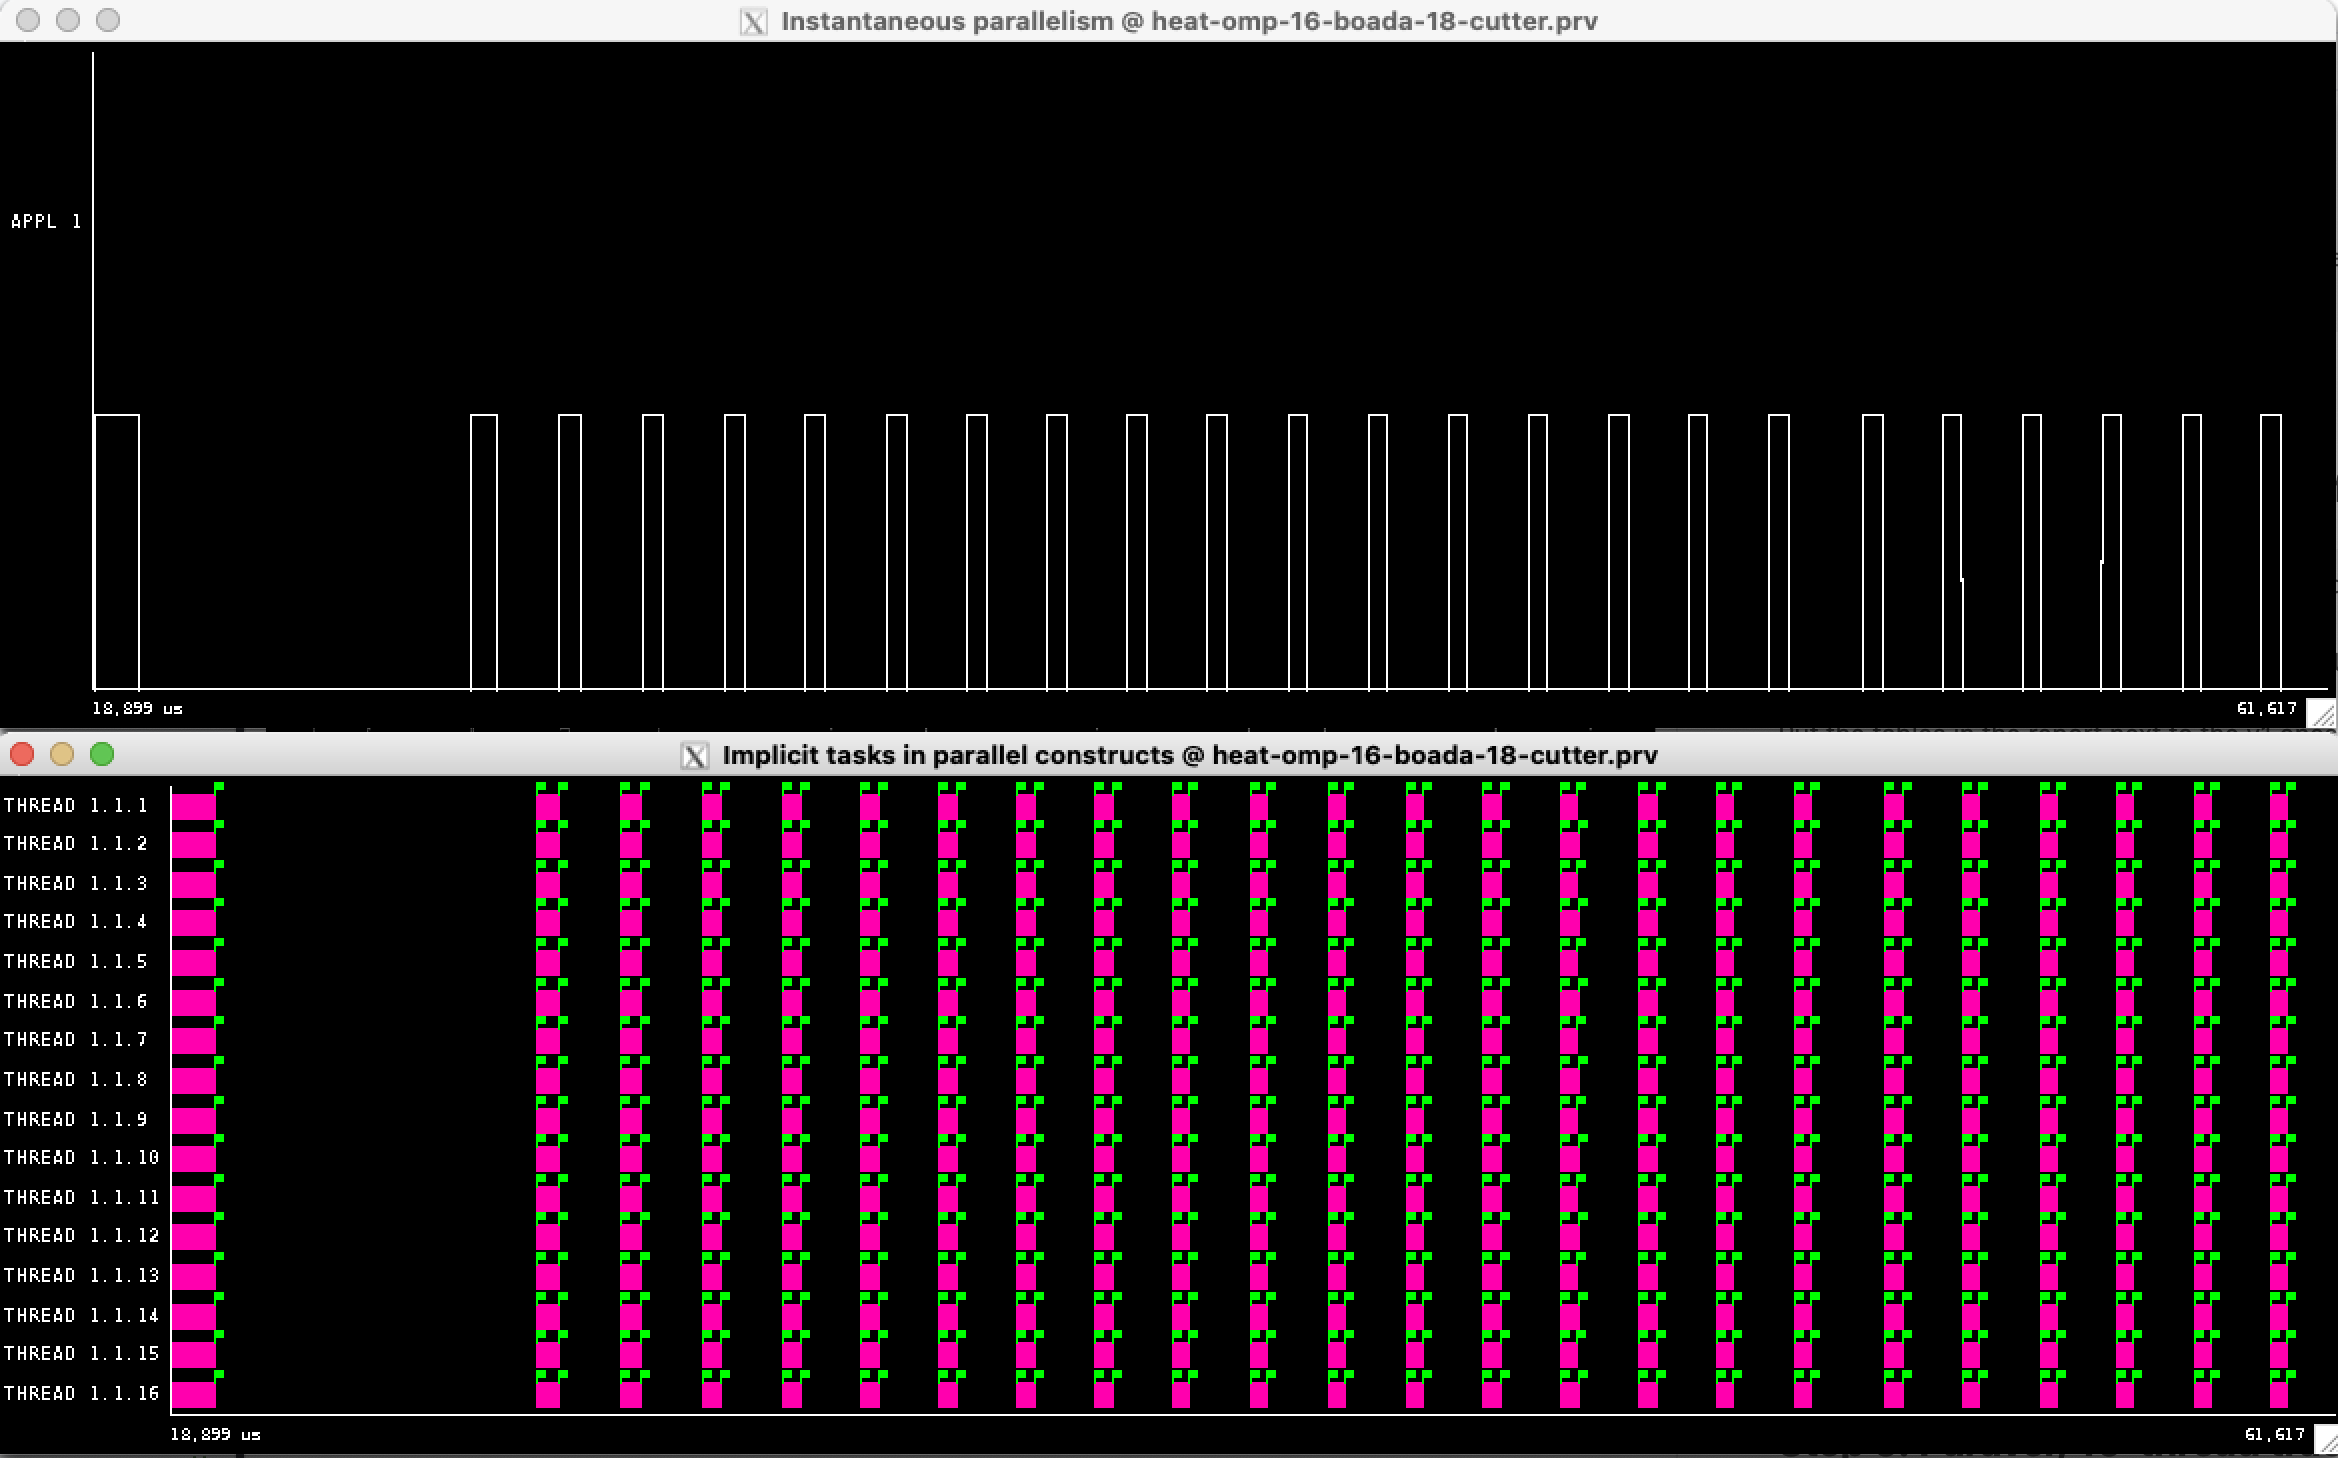
\includegraphics[width=\textwidth]{heat-omp-16-boada-18-cutter-v1.png}
  \caption{v1, 16 threads. Narrow pulses: parallel \texttt{solve} (all 16 threads). Wide gaps: sequential \texttt{copy\_mat}, with instantaneous parallelism equal to 1.}
  \label{fig:paraver-v1}
\end{figure}

Each iteration of about 1.5\,ms has two parts:
\begin{itemize}
  \item a short parallel region of about 0.5\,ms, in which all 16 threads execute \texttt{solve} and the instantaneous parallelism is 16;
  \item a gap of about 1\,ms, in which only the master thread runs and the instantaneous parallelism drops to 1.
\end{itemize}
The pulses are clean squares with no staircase at the end, so the load is well balanced (load balancing 99.9\%). The longer gap after the first pulse is the warm-up of the first iteration.

\textbf{Which region causes the low parallel fraction?} It is what happens between two consecutive calls to the solver: \texttt{copy\_mat(param.uhelp, param.u, np, np)} in \texttt{heat-omp.c}, which copies the new matrix back into \texttt{u} sequentially. With 16 threads, this serial gap is about twice as long as the parallel part. This is exactly what Tareador predicted for version J2, where \texttt{copy\_mat} was the only task running between the parallel \texttt{solve} phases.

\subsection{Optimisation}

We parallelised \texttt{copy\_mat} with the same row decomposition as \texttt{solve} (version \textbf{v2}):

\begin{lstlisting}
void copy_mat (double *u, double *v, unsigned sizex, unsigned sizey) {
    #pragma omp parallel
    {
        int myid = omp_get_thread_num();
        int nthr = omp_get_num_threads();
        int i_start = lowerb(myid, nthr, sizex);
        int i_end   = upperb(myid, nthr, sizex);

        for (int i = max(1, i_start); i <= min(sizex - 2, i_end); i++)
            for (int j = 1; j < sizey - 1; j++)
                v[i * sizey + j] = u[i * sizey + j];
    }
}
\end{lstlisting}

The copied rows are independent (Tareador version J3), so no synchronisation is needed inside the region. Using the \emph{same} decomposition matters: thread $k$ copies exactly the rows it has just computed in \texttt{solve} (owner-computes rule), so the data is still in its own cache. With 16 threads, each thread's part of \texttt{u} and \texttt{uhelp} is about 1\,MB, which fits in its 1.25\,MB L2 cache. We validated v2 with 16 threads; the image is identical to the sequential one.

\subsubsection{Overall analysis of the optimised code}

\begin{table}[H]
\centering
\small
\begin{tabular}{|l|c|c|c|c|}
\hline
\multicolumn{5}{|c|}{Overview of whole program execution metrics} \\
\hline
\hline
Number of processors & 1 & 4 & 8 & 16 \\
\hline
Elapsed time (sec)      &       2.36 &       0.65 &       0.37 &       0.20 \\
\hline
Speedup                 &       1.00 &       3.63 &       6.30 &      11.78 \\
\hline
Efficiency              &       1.00 &       0.91 &       0.79 &       0.74 \\
\hline
\end{tabular}
\vspace{2mm}
\begin{tabular}{|l|c|c|c|c|}
\hline
\multicolumn{5}{|c|}{Overview of the Efficiency metrics in parallel fraction, $\phi$=98.74\%} \\
\hline
\hline
Number of processors & 1 & 4 & 8 & 16 \\
\hline
\hline
Global efficiency                      &     99.81\% &     93.75\% &     83.71\% &     83.28\% \\
\hline
\hline
Parallelization strategy efficiency &     99.81\% &     95.36\% &     95.67\% &     93.27\% \\
\hline
Load balancing                   &    100.00\% &     96.68\% &     98.68\% &     98.66\% \\
In execution efficiency          &     99.81\% &     98.63\% &     96.95\% &     94.53\% \\
\hline
\hline
Scalability for computation tasks   &    100.00\% &     98.32\% &     87.50\% &     89.29\% \\
\hline
IPC scalability                  &    100.00\% &     98.52\% &     90.25\% &     93.92\% \\
Instruction scalability          &    100.00\% &     99.96\% &     97.73\% &     96.80\% \\
Frequency scalability            &    100.00\% &     99.84\% &     99.20\% &     98.21\% \\
\hline
\end{tabular}
\vspace{2mm}
\begin{tabular}{|l|c|c|c|c|}
\hline
\multicolumn{5}{|c|}{Statistics about implicit or explicit tasks in parallel fraction} \\
\hline
\hline
Number of processors & 1 & 4 & 8 & 16 \\
\hline
\hline
Number of implicit tasks per thread (average us)    &          2000.0 &          2000.0 &          2000.0 &          2000.0 \\
\hline
Useful duration for implicit tasks (average us)     &         1163.62 &          295.87 &          166.23 &           81.45 \\
\hline
Load balancing for implicit tasks                &             1.0 &            0.97 &            0.99 &            0.99 \\
\hline
Time in synchronization implicit tasks (average us) &             0.0 &             0.0 &             0.0 &             0.0 \\
\hline
Time in fork/join implicit tasks (average us)       &            2.26 &           21.43 &             8.6 &            7.58 \\
\hline
\end{tabular}

\caption{\texttt{modelfactors} for v2 (parallel \texttt{solve} and \texttt{copy\_mat}).}
\label{tab:mf-v2}
\end{table}

\begin{figure}[H]
  \centering
  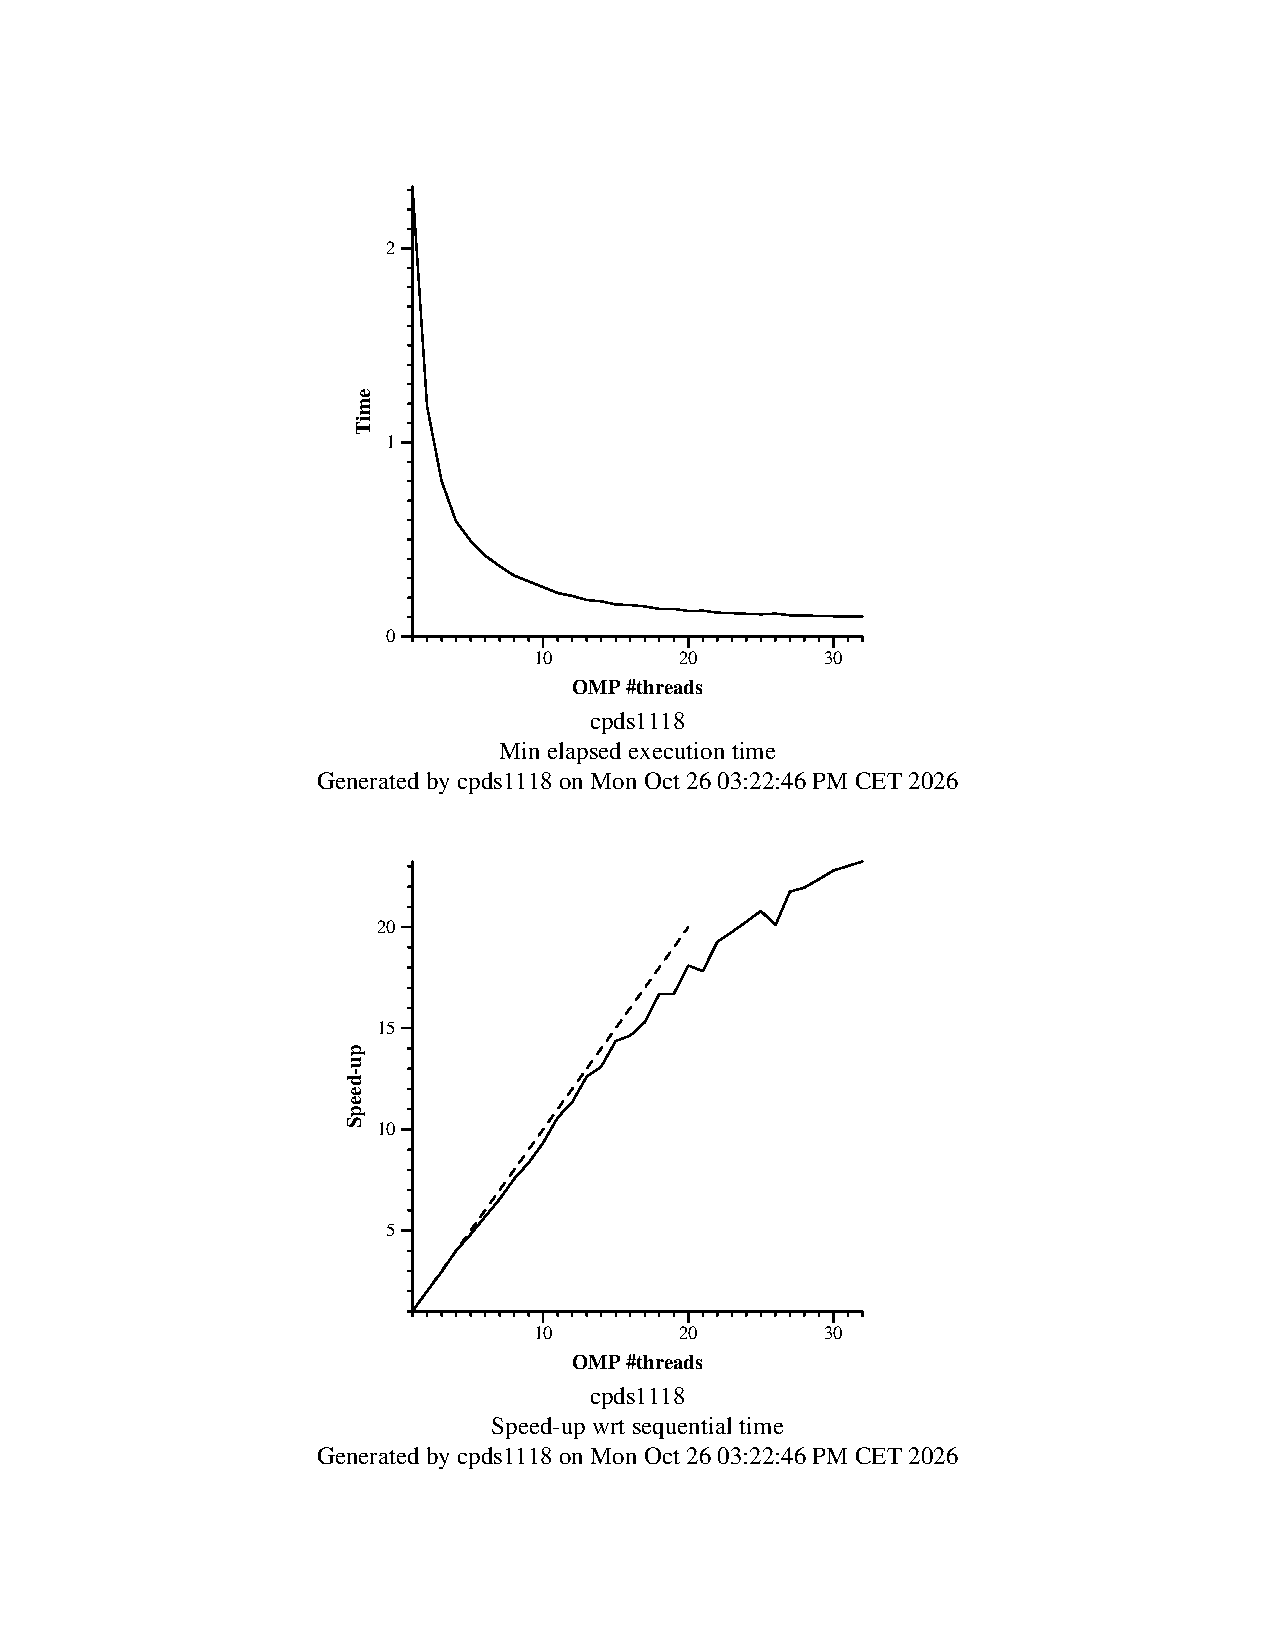
\includegraphics[width=0.55\textwidth, trim=0 60 0 60, clip]{strong-heat-omp-jacobi-1-32-3-boada-18-v2.pdf}
  \caption{Strong scalability of v2 (\texttt{submit-strong-omp.sh}, Jacobi, 1 to 32 threads).}
  \label{fig:strong-v2}
\end{figure}

\begin{table}[H]
\centering
\begin{tabular}{lrrr}
\toprule
 & v1 & v2 & v2 vs v1 \\
\midrule
Parallel fraction $\phi$ & 73.59\% & 98.74\% & \\
Elapsed time, 16 threads & 1.54 s & 0.20 s & $7.7\times$ faster \\
Speedup, 16 threads & 1.56 & 11.78 & \\
Efficiency, 16 threads & 0.10 & 0.74 & \\
IPC scalability, 16 threads & 42.75\% & 93.92\% & \\
\bottomrule
\end{tabular}
\caption{Comparison of the first implementation (v1) and the optimised one (v2).}
\label{tab:v1v2}
\end{table}

\begin{itemize}
  \item \textbf{Is the execution time reduced?} Yes. On 16 threads it drops from 1.54\,s (v1) to 0.20\,s (v2).
  \item \textbf{Has the scalability increased?} Yes. The speedup grows with the number of threads (3.63, 6.30 and 11.78 on 4, 8 and 16), and the strong-scalability plot (Figure~\ref{fig:strong-v2}) stays close to the ideal line up to about 12 threads, reaching about 23 on 32 threads. Beyond that point the gap to the ideal grows because the threads share the memory bandwidth (the stencil performs 5 loads and 1 store for every 4 additions). The plot measures a higher speedup than \texttt{modelfactors} (about 14.5 against 11.78 on 16 threads) because those executions are not instrumented and the script keeps the best of 3 runs. As the assignment notes, \texttt{time} is not very precise.
  \item \textbf{Is the parallel fraction larger?} Yes, it rises from 73.59\% to 98.74\%. The remaining 1.3\% is the control of the \texttt{while} loop and the initialisation.
  \item \textbf{Speedup with respect to the first implementation on 16 threads:} $1.54 / 0.20 \approx 7.7\times$.
\end{itemize}

The other metrics are also good. Load balancing is 98.7\% and the IPC scalability rises from 42.8\% to 93.9\%, because each thread now keeps its rows in its own cache. The time in fork/join per thread is small (7.6\,$\mu$s), even though there are now two parallel regions per iteration (2\,000 implicit tasks per thread).

\subsubsection{Detailed analysis of the optimised code}

\begin{figure}[H]
  \centering
  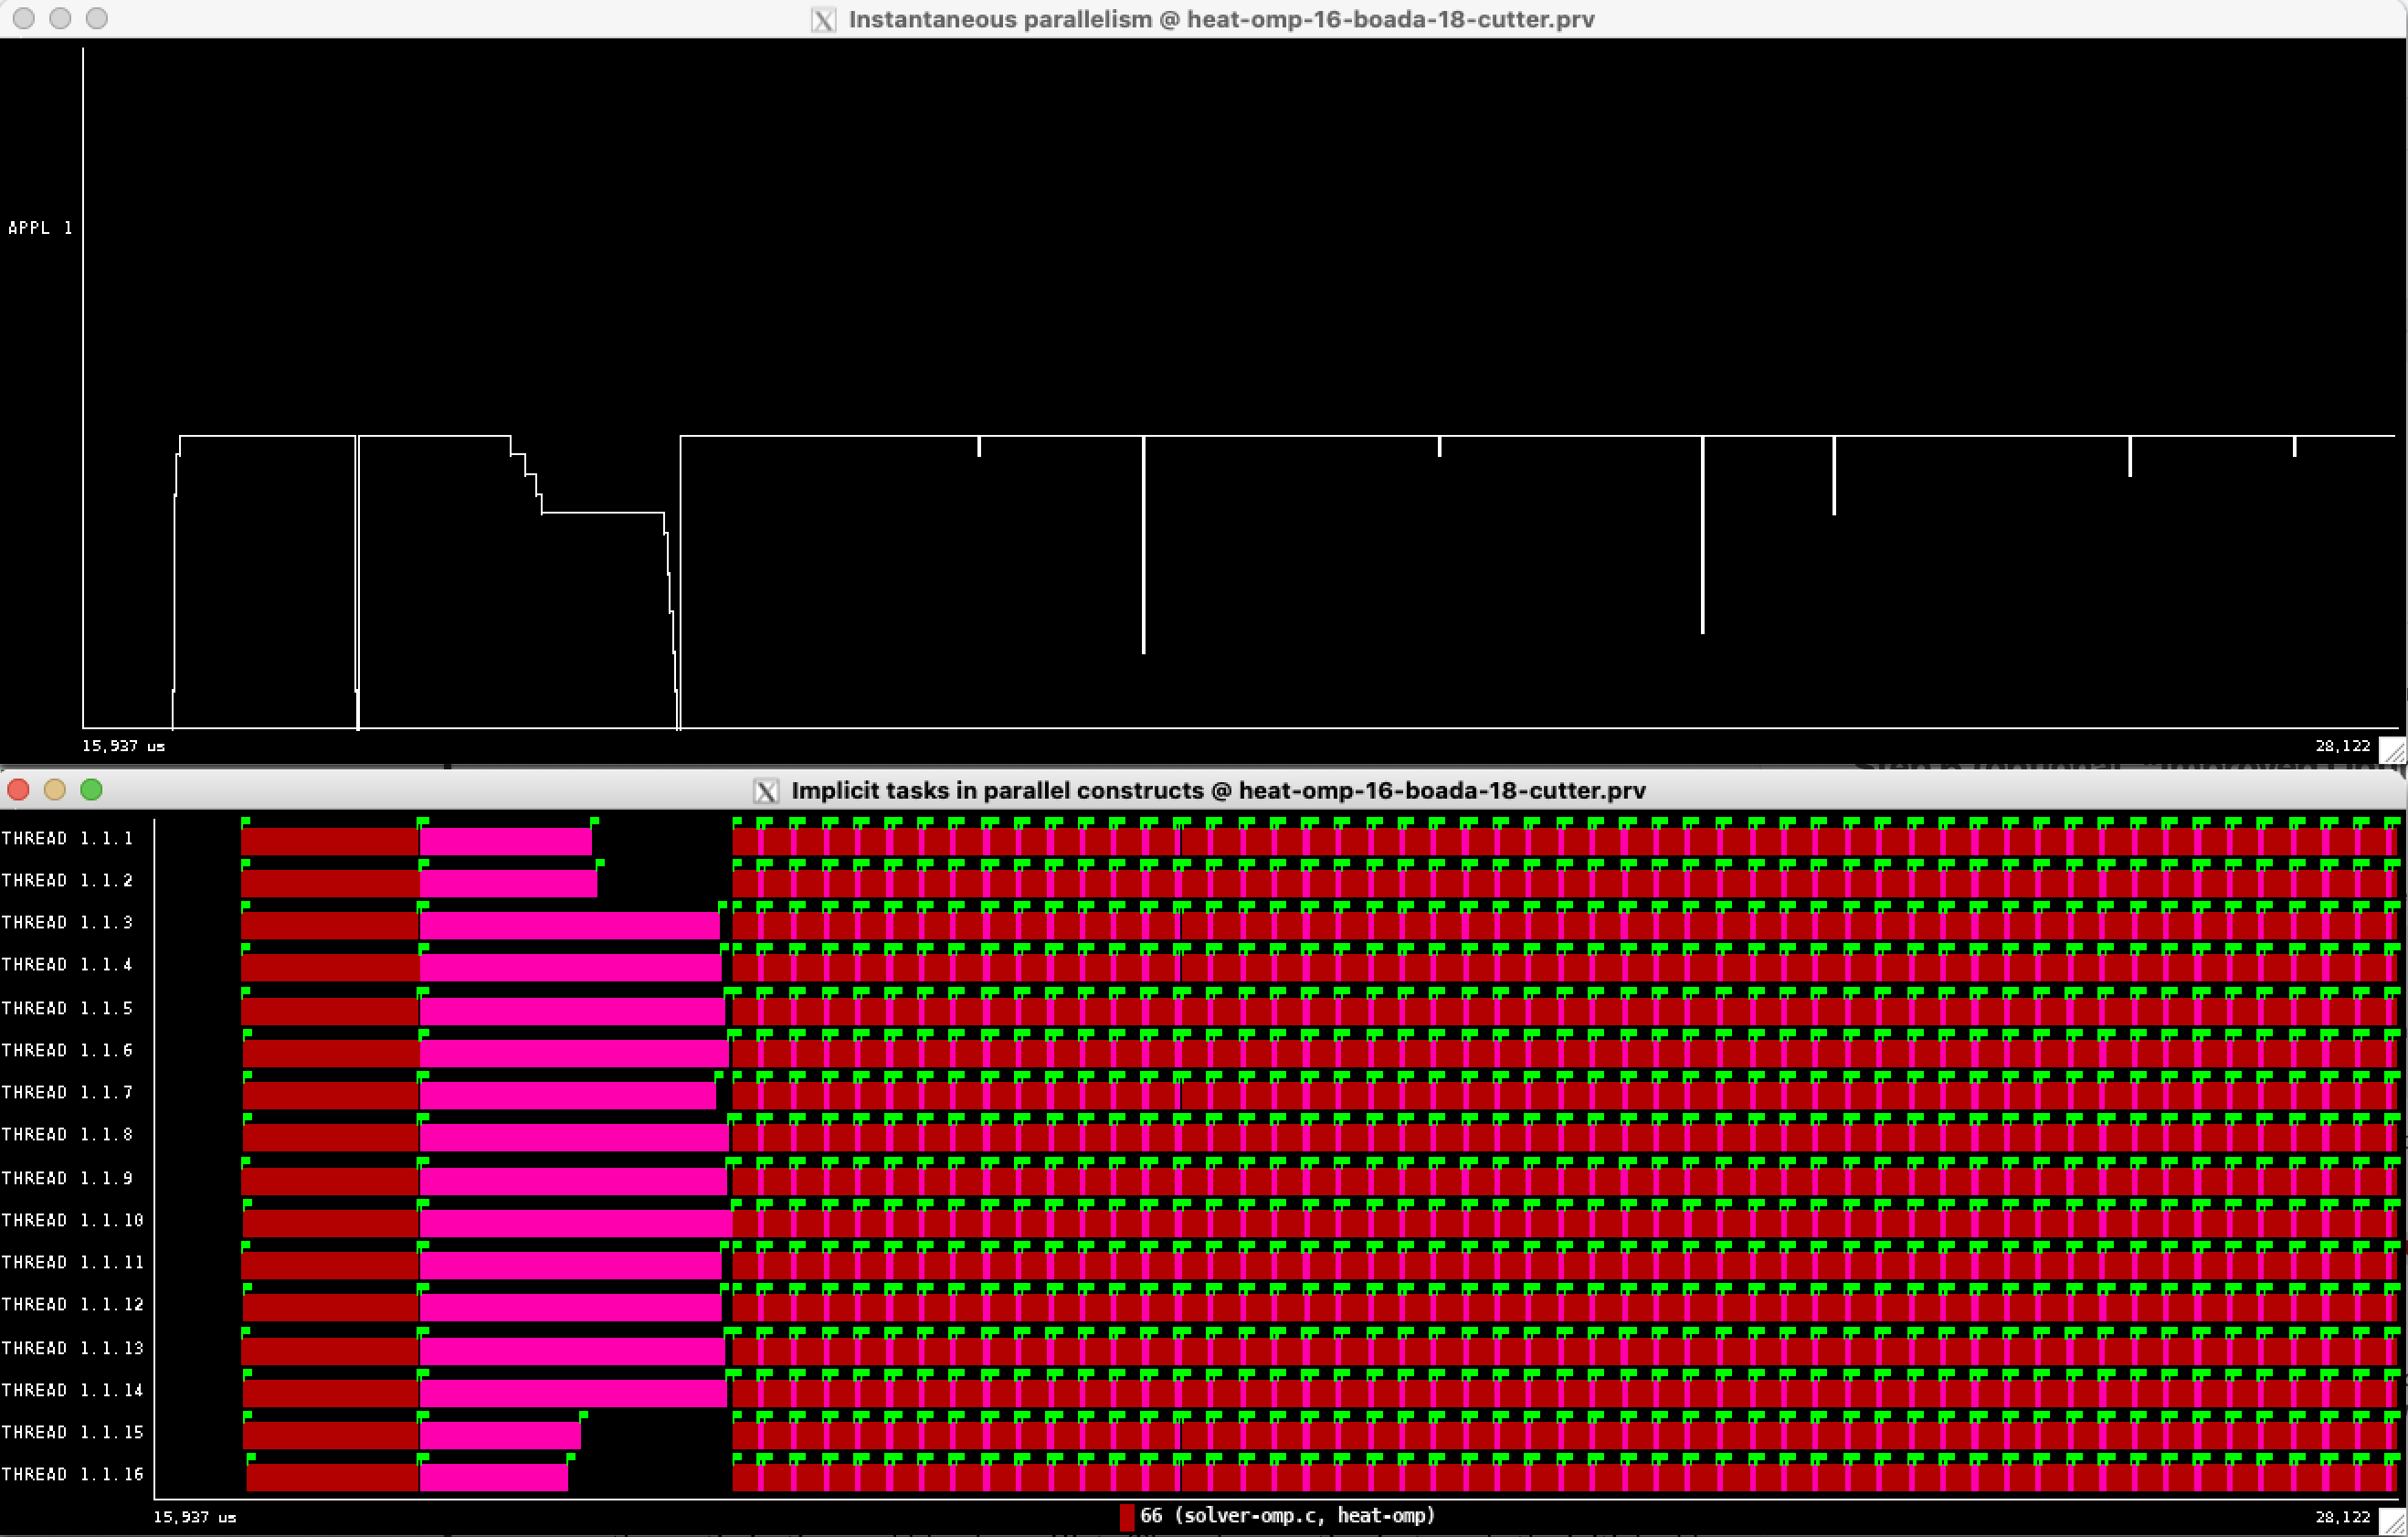
\includegraphics[width=\textwidth]{heat-omp-16-boada-18-cutter-v2.png}
  \caption{v2, 16 threads: \texttt{solve} (dark red) and the parallel \texttt{copy\_mat} (magenta) alternate with only thin barriers between them. The left part is the first iteration (warm-up).}
  \label{fig:paraver-v2}
\end{figure}

In Figure~\ref{fig:paraver-v2}, after the first iteration, the two parallel regions of each iteration alternate on all 16 threads, and the instantaneous parallelism stays at 16 almost all the time, with only a few short drops at the barriers. About 50 iterations fit in 12\,ms (about 0.23\,ms per iteration, consistent with 0.20\,s for 1\,000 iterations), compared with about 1.5\,ms per iteration in v1. The sequential gaps of Figure~\ref{fig:paraver-v1} have disappeared. The first iteration is slower and less balanced (some threads finish the first copy early) because the caches are still cold and memory pages are touched for the first time.

\paragraph{Further optimisation (not implemented).}
\texttt{copy\_mat} only moves the new values back into \texttt{u}. Since \texttt{solve} only needs the addresses of the input and output matrices, the copy could be removed completely by swapping the \texttt{u} and \texttt{uhelp} pointers after each iteration. This replaces $O(N^2)$ work with $O(1)$ work and removes one parallel region and its barrier per iteration. It is safe because \texttt{uhelp} is initialised as a full copy of \texttt{u}, so both matrices hold the same boundary values. We have not implemented this version.

\end{document}
